% This is LLNCS.DOC the documentation file of
% the LaTeX2e class from Springer-Verlag
% for Lecture Notes in Computer Science, version 2.4
\documentclass{llncs}
\usepackage{llncsdoc}

%\usepackage{a4wide}

\usepackage{graphicx}
\usepackage{verbatim}


\let\proof\relax   
\let\endproof\relax

\usepackage{amsmath,amsthm,amscd}
\usepackage{amssymb}    % for blackboard B
\usepackage{rotating}   % to rotate the figures
\usepackage{mathpartir} % math paragraph + inference rules
\usepackage{mathtools}  % for align, multline etc.
\usepackage{caption}
\usepackage{xifthen}
\usepackage{stmaryrd} % double brackets (\llbracket, \rrbracket)

%% \usepackage[justification=centering,belowskip=-10pt,aboveskip=0pt]{caption}
%% \setlength{\intextsep}{10pt plus 2pt minus 2pt}
%% \setlength\abovedisplayskip{0pt}

\usepackage{wrapfig}
\usepackage{subcaption}
\usepackage{hyperref}

% Simon's macros for the BIPspec-ArchFailureTimerMax diagrams
\newcommand{\cstate}[1]{\ensuremath{s_{#1}}}
\newcommand{\tstate}[1]{\ensuremath{t_{#1}}}

\newcommand{\NameCtrl}{\ensuremath{\mathit{Ctrl}}}
\newcommand{\NameTimer}{\ensuremath{\mathit{Timer}}}
\newcommand{\NameOprnd}{\ensuremath{B}}

\newcommand{\PortFinish}{\ensuremath{\mathsf{finish}}}
\newcommand{\PortFail}{\ensuremath{\mathsf{fail}}}
\newcommand{\PortResume}{\ensuremath{\mathsf{resume}}}
\newcommand{\PortReset}{\ensuremath{\mathsf{reset}}}
\newcommand{\PortTO}{\ensuremath{\mathsf{timeout}}}
\newcommand{\PortStart}{\ensuremath{\mathsf{start}}}
\newcommand{\PortTick}{\ensuremath{\mathsf{tick}}}
\newcommand{\PortCancel}{\ensuremath{\mathsf{resume}}}
\newcommand{\PortAsk}{\ensuremath{\mathsf{ask}}}

\newcommand{\TimerInit}[1][\!]{\ensuremath{t {#1}:={#1} 0}}
\newcommand{\TimerInitZone}[1][\!]{\ensuremath{z {#1}:={#1} [0,0], t {#1}:={#1} 0}}
\newcommand{\TimerUpd}[1][\!]{\ensuremath{t {#1}:={#1} t {#1}+{#1} 1}}
\newcommand{\GuardTick}[1][\!]{\ensuremath{[t {#1}<{#1} z.u]}}
\newcommand{\GuardTO}[1][\!]{\ensuremath{[t {#1}\in{#1} \mathit{z}]}}

\newcommand{\InitTransfer}[1][\!]{\ensuremath{\NameTimer.\mathit{z} {#1}:={#1} \NameCtrl.\mathit{zone}}}
\newcommand{\IntervalInit}[1][\!]{\ensuremath{\mathit{zone} {#1}:={#1} [\mathrm{Min}, \mathrm{Max}]}}
         % Definitions of macros used in XFig figures

\usepackage{soul}
\usepackage[colorinlistoftodos,bordercolor=white]{todonotes}
%% \usepackage[disable,colorinlistoftodos,bordercolor=white]{todonotes}
\usepackage{macrospNets}

\newcommand{\Simon}{\\\hfill\mdash Simon}

\newcommand{\noteSB}[2][color=green!40, size=\tiny]{\todo[#1]{{#2}\Simon}}
\newcommand{\noteSBin}[2][inline,color=green!40]{\todo[#1]{{#2}\Simon}}
\newcommand{\todoSB}[2][color=green!40, size=\tiny]{\todo[#1]{\textbf{To-do Simon:} {#2}}}
\newcommand{\todoSBin}[2][inline,color=green!40]{\todo[#1]{\textbf{To-do Simon: } {#2}}}
\newcommand{\Ludo}{\\\hfill\mdash Ludo}
\newcommand{\noteLH}[2][color=orange!40, size=\tiny]{\todo[#1]{{#2}\Ludo}}
\newcommand{\noteLHin}[2][inline,color=orange!40]{\todo[#1]{{#2}\Ludo}}
\newcommand{\todoLH}[2][color=orange!40, size=\tiny]{\todo[#1]{\textbf{To-do Ludo:} {#2}}}
\newcommand{\todoLHin}[2][inline,color=orange!40]{\todo[#1]{\textbf{To-do Ludo: } {#2}}}

\newcommand{\noteIn}[2][inline,color=black!20]{\todo[#1]{{#2}}}

\newcommand{\add}[2][Added]{\todo[color=blue!20, size=\tiny]{#1}{\color{blue}#2}}
%% \newcommand{\remove}[2][Removed]{\todo[color=red!20, size=\tiny]{#1}}
\newcommand{\remove}[2][Removed]{\todo[color=red!20, size=\tiny]{#1}{\color{red}\st{#2}}}
\newcommand{\removeIn}[2][Removed]{\todo[color=red!10, inline]{{\color{red}#2}#1}}
%% \newcommand{\replace}[3][Replaced]{\todo[color=blue!20, size=\tiny]{#1}{\color{blue}#3}}
\newcommand{\replace}[3][Replaced]{\todo[color=blue!20, size=\tiny]{#1}{\color{blue}#3}{\color{red}\st{#2}}}

\newcommand{\addSB}[1]{\add[Added by Simon]{#1}}
\newcommand{\removeSB}[1]{\remove[Removed by Simon]{#1}}
\newcommand{\removeSBin}[1]{\removeIn[Removed by Simon]{#1}}
\newcommand{\replaceSB}[2]{\replace[Replaced by Simon]{#1}{#2}}

\newcommand{\defn}[1]{Def.~\ref{defn:#1}}
\newcommand{\defntwo}[2]{Defs~\ref{defn:#1} and \ref{defn:#2}}
\newcommand{\fig}[1]{Fig.~\ref{fig:#1}}
\newcommand{\figs}[2]{Fig.~\ref{fig:#1} and~\ref{fig:#2}}
\newcommand{\tab}[1]{Tab.~\ref{tab:#1}}
\newcommand{\eq}[1]{(\ref{eq:#1})}
\newcommand{\res}[1]{(\ref{res:#1})}
\newcommand{\ex}[1]{Ex.~\ref{ex:#1}}
\newcommand{\exs}[2]{Ex.~\ref{ex:#1} and~\ref{ex:#2}}
\newcommand{\secn}[1]{Sect.~\ref{secn:#1}}
\newcommand{\rem}[1]{Note~\ref{rem:#1}}
\newcommand{\lem}[1]{Lem.~\ref{lem:#1}}
\newcommand{\cor}[1]{Cor.~\ref{cor:#1}}
\newcommand{\thm}[1]{Th.~\ref{thm:#1}}
\newcommand{\axs}[1]{Ax.~\ref{ax:#1}}
% \newcommand{\ax}[2]{\ref{ax:#1}.\ref{ax:#1:#2}}
\newcommand{\ax}[1]{Ax.~\ref{ax:#1}}
\newcommand{\prop}[1]{Prop.~\ref{prop:#1}}
\newcommand{\alg}[1]{Alg.~\ref{alg:#1}}
\newcommand{\asmp}[1]{Ass.~\ref{asmp:#1}}

% %%%%%%%%%%%%%%%%%%%%%

\newcommand{\cA}{\ensuremath{\mathcal{A}}}
\newcommand{\fA}{\ensuremath{\mathsf{A}}}
\newcommand{\sA}{\ensuremath{\mathbb{A}}}
\newcommand{\cB}{\ensuremath{\mathcal{B}}}
\newcommand{\fB}{\ensuremath{\mathsf{B}}}
\newcommand{\sB}{\ensuremath{\mathbb{B}}}
\newcommand{\cC}{\ensuremath{\mathcal{C}}}
\newcommand{\sC}{\ensuremath{\mathbb{C}}}
\newcommand{\cD}{\ensuremath{\mathcal{D}}}
\newcommand{\fD}{\ensuremath{\mathsf{D}}}
\newcommand{\sD}{\ensuremath{\mathbb{D}}}
\newcommand{\cE}{\ensuremath{\mathcal{E}}}
\newcommand{\sE}{\ensuremath{\mathbb{E}}}
\newcommand{\cF}{\ensuremath{\mathcal{F}}}
\newcommand{\cG}{\ensuremath{\mathcal{G}}}
\newcommand{\cH}{\ensuremath{\mathcal{H}}}
\newcommand{\cI}{\ensuremath{\mathcal{I}}}
\newcommand{\sI}{\ensuremath{\mathbb{I}}}
\newcommand{\cM}{\ensuremath{\mathcal{M}}}
\newcommand{\cN}{\ensuremath{\mathcal{N}}}
\newcommand{\sN}{\ensuremath{\mathbb{N}}}
\newcommand{\cP}{\ensuremath{\mathcal{P}}}
\newcommand{\sP}{\ensuremath{\mathbb{P}}}
\newcommand{\cQ}{\ensuremath{\mathcal{Q}}}
\newcommand{\sQ}{\ensuremath{\mathbb{Q}}}
\newcommand{\cR}{\ensuremath{\mathcal{R}}}
\newcommand{\sR}{\ensuremath{\mathbb{R}}}
\newcommand{\cS}{\ensuremath{\mathcal{S}}}
\newcommand{\sS}{\ensuremath{\mathfrak{S}}}
\newcommand{\cT}{\ensuremath{\mathcal{T}}}
\newcommand{\fT}{\ensuremath{\mathsf{T}}}
\newcommand{\sT}{\ensuremath{\mathbb{T}}}
\newcommand{\cV}{\ensuremath{\mathcal{V}}}
\newcommand{\fV}{\ensuremath{\mathsf{V}}}
\newcommand{\sV}{\ensuremath{\mathbb{V}}}
\newcommand{\sZ}{\ensuremath{\mathbb{Z}}}

\newcommand{\mdash}[1][]{---#1}
\newcommand{\ndash}{--}
\newcommand{\ie}[1][\ ]{i.e.#1}
\newcommand{\etc}[1][\ ]{etc.#1}
\newcommand{\eg}[1][\ ]{e.g.#1}
\newcommand{\cf}[1][\ ]{cf.#1}
\newcommand{\wrt}[1][\ ]{w.r.t.#1}
\newcommand{\resp}[1][\ ]{resp.#1}

\newcommand{\bydef}[1]{\ensuremath{\stackrel{\mathit{\scriptscriptstyle def}}{#1}}}
\newcommand{\suchthat}{\ensuremath{\,|\,}}
\newcommand{\rightsuchthat}{\ensuremath{\,\right|\,}}
\newcommand{\leftsuchthat}{\ensuremath{\,\left|\,}}
\newcommand{\setdef}[2]{\ensuremath{\{{#1}\,|\,{#2}\}}}
\newcommand{\setdefb}[2]{\ensuremath{\bigl\{{#1}\,\bigl|\,{#2}\bigr.\bigr\}}}
\newcommand{\Setdef}[2]{\ensuremath{\Big\{{#1}\,\Big|\,{#2}\Big\}}}
\newcommand{\goesto}[2][]{\ensuremath{\xrightarrow[#1]{#2}}}
\newcommand{\notgoesto}[2][]{\ensuremath{\not\xrightarrow[#1]{\ \,#2}}}
\newcommand{\non}[1]{\ensuremath{\overline{#1}}}

\newcommand{\true} {\ensuremath{\mathtt{t\!t}}}
\newcommand{\false}{\ensuremath{\mathtt{f\!f}}}
\newcommand{\noop} {\ensuremath{\emptyset}} % \mathsf{skip}

\newcommand{\ordbool}{\ensuremath{\sB^{<}}}
\newcommand{\data}{\ensuremath{\sD}}
\newcommand{\signature}{\ensuremath{\Sigma}}
\newcommand{\variables}{\ensuremath{\cV}}
\newcommand{\Talg}{\ensuremath{\cT_{\signature,\variables}}}
\newcommand{\actions}[1]{\ensuremath{\cA_{#1}}}
\newcommand{\guards}[1]{\ensuremath{\ordbool_{#1}}}
\newcommand{\exprs}[1]{\ensuremath{\sE_{#1}}}
\newcommand{\boolexprs}[1]{\ensuremath{\sB_{#1}}}
\newcommand{\assigns}[1]{\ensuremath{\sA_{#1}}}
\newcommand{\valuations}[1]{\ensuremath{\data^{#1}}}
\newcommand{\val}[3][]{\ensuremath{#1{\sigma}^{#2}_{#3}}}

\newcommand{\filter}[2][]{\ensuremath{\pi_{#1}({#2})}}

\newcommand{\primeit}[1]{#1'}
\newcommand{\doubleprimeit}[1]{#1''}


\newcommand{\export}[1][]{\ensuremath{\varepsilon_{#1}}}
\newcommand{\valdiff}[2]{\ensuremath{#1 \triangle #2}}
\newcommand{\supp}[1]{\ensuremath{\mathrm{supp}(#1)}}
\newcommand{\semopen}[1]{\ensuremath{[{#1}]}}
\newcommand{\semclosed}[1]{\ensuremath{\llbracket{#1}\rrbracket}}
\newcommand{\reachable}[1]{\ensuremath{\mathit{reachable}({#1})}}
\newcommand{\IMextend}[2]{\ensuremath{#1 \ltimes #2}}
\newcommand{\arcomp}{\oplus}
\newcommand{\arequiv}{\equiv}
\newcommand{\Arcomp}{\Bigoplus}
\newcommand{\expmix}{\wedge}
\newcommand{\order}{\leqslant}

\makeatletter
\newcommand{\doubletilde}[1]{{%
  \mathpalette\double@tilde{#1}%
}}
\newcommand{\double@tilde}[2]{%
  \sbox\z@{$\m@th#1\tilde{#2}$}%
  \ht\z@=.9\ht\z@
  \tilde{\box\z@}%
}
\makeatother

\newcounter{tempctr}
\newcommand{\breakenumistart}{%
  \setcounter{tempctr}{\value{enumi}}%
  \end{enumerate}%
}
\newcommand{\breakenumiend}{%
  \begin{enumerate}%
  \setcounter{enumi}{\value{tempctr}}%
}

% %%%%%%%%%%%%%%%%%%%%%

\usepackage{tikz}
\usetikzlibrary{calc}
\usetikzlibrary{arrows,shapes,automata,petri}
  \tikzset{
  place/.style={
    circle,
    thick,
    draw=blue!75,
    fill=blue!20,
    minimum size=6mm
  },
  transition/.style={
    rectangle,
    thick,
    fill=black,
    minimum width=8mm,
    inner ysep=2pt
    },
    arc/.style = {
      decoration=
      {markings,mark=at position #1 with {circle;}
      },
      postaction={decorate,draw}},
  }   

\let\llncssubparagraph\subparagraph
\let\subparagraph\llncssubparagraph

\begin{document}
\graphicspath{{figures/}}

\title{Architectures and Open pNets}

\author{%
Simon~Bliudze\inst{1}
\and
Ludovic~Henrio\inst{2}
\and
Eric~Madelaine\inst{3}
\and
...
}

\institute{%
  INRIA Lille -- Nord Europe, Villeneuve d'Ascq, France\\
  \email{simon.bliudze@inria.fr}
\and
\and
}


\maketitle

\begin{abstract}
  We extend the theory of architectures with a general
  mechanism for handling various types of data transfer.  We
  encode this extended model into the open pNet semantic
  model and show how this encoding can be used to verify
  that an architecture does, indeed, enforce its
  characteristic property.

\keywords{}
\end{abstract}

%****************************************************************
%****************************************************************

\section{Introduction}
\label{secn:introduction}

BIP (Behaviour-Interaction-Priority)~\cite{bip} is a framework for the
component-based design of concurrent software and systems.  In
particular, the BIP tool-set comprises compilers for generating C/C++
code, executable by linking with one of the dedicated engines, which
implement the BIP operational semantics~\cite{BliSif08-acp-tc}.
This approach ensures that any property, shown to hold on a given BIP
model, will also hold by construction on the generated code.

In this context, the notion of \emph{architecture} was proposed
in~\cite{AttieBBJS16-architectures-faoc} as a mechanism for ensuring
correctness by construction during the design of BIP models.
Architectures can be viewed as operators transforming BIP models.
They formalise design patterns, which enforce global properties
characterising the coordination among the components of the system.
The architecture-based design process in BIP takes as input a set of
components providing basic functionality of the system and a set of
temporal properties that must be enforced in the final system.  For
each property, a corresponding architecture is identified
%% \footnote{%
%% %
%%   The current approach relies on taxonomies of predefined
%%   architectures.  Future work may include automatic synthesis of
%%   architectures from, \eg CTL~\cite{BaierKatoen2008} formulae.
%% %
%% }
and applied to the model, thereby potentially introducing additional
coordinator components and modifying the connectors that define
synchronisation patterns among ports of components.
In~\cite{AttieBBJS16-architectures-faoc}, it was shown that
application of architectures is compositional \wrt safety properties,
\ie when several architectures are applied, each enforcing a safety
property, the resulting system satisfies their conjunction.

The concepts and results of the paper are illustrated by a running
example extending the Failure Monitor architecture from the CubETH
nanosatellite on-board software case-study~\cite{CubETH-case-study}.

%****************************************************************
%****************************************************************

\section{Preliminaries}
\label{secn:preliminaries}

%****************************************************************

\subsection{Notations}
\label{secn:notations}

We extensively use indexed structures
over some countable indexed sets, which are equivalent to mappings over
the countable set. 
Thus, 
$a_i^{i\in I}$
%, or equivalently  $(i\mapsto a_i)^{i\in I}$
denotes a family of elements $a_i$ indexed over the
set $I$. % Such a family
% is equivalent to the mapping $(i\mapsto a_i)^{i\in I}$.
% To specify the set over which the structure is indexed,
% indexed structures are always denoted with an exponent of the form $i\in I$
% (arithmetic only appears in the indexes if necessary).
This notation defines both $I$ the set over which the family is
indexed (called \emph{range}), and $a_i$ the elements of the family.
E.g., $a^{i\in\{3\}}$ is the mapping with a single entry $a$ at index
$3$ ; abbreviated $(3\mapsto a)$ in the following.
When this is not
ambiguous, we shall use notations for sets, and typically write
``indexed set over I'', even though formally we should speak of multisets; and
write $x\in a_i^{i\in I}$ to mean $\exists i\in I.\, x=a_i$.  An empty
family is denoted $\emptyset$. We use a classical overline notation, \eg $\overline{a}$, 
for a family, where the indexing set is irrelevant. Finally, we use $\uplus$ to denote 
the disjoint union on
indexed sets.

\noteIn{states looks ok, but initial state is $s_0$ in pNet and not in archi : $s^0$.  Exponent 
position was removed from pNet because we found it complex with indexed set notation but 
could be ok.
\Ludo

I am using exponent notation for ``modifiers'', reserving\mdash
as much as possible\mdash index notation for enumeration.  I
think this can be solved, where necessary, by using parentheses,
\eg $(s^0_i)^{i \in I}$
\Simon
}

%****************************************************************

\subsection{Term algebra}
\label{secn:terms}

\todoLHin{Remove term algebra or simplify?}
\todoLHin{universal domain $\implies$ remove sort}
\todoLHin{replace assignments by $e_i$

  In fact, in the pNet action terms, you need expressions, not
  assignements.  Therefore assuming that all expressions are
  assignments will not work, so the right approach is to have
  expressions (for pNets) and assignments (for BIP) separately.
  \Simon
%
}

\noteSBin{In Archi we have $a$, whereas in pNets we have $\alpha$, where, approximately $\alpha = 
a(x_1..x_n)$, except that $a$ is port name in archi and action name in pNets.
Is this true? can we unify better? or is it sufficient?
\Ludo

$a$ is a set of ports, but otherwise, yes, this is true.  I think
this is coherent, since, in archi, we have the ``interaction
part'', \ie only ports, plus the data part, \ie variables,
guards, expressions.  In pNets, these are combined.  So, it seems
ok that notations differ\mdash ``uniformisation'' will be
achieved by encoding archi $\rightarrow$ pNets.
}

\noteLHin{I believe we should simplify this paragraph about param actions}
The pNet model in \secn{pNets} relies on a notion of parameterised actions, that are
symbolic expressions using data types and variables. As we aim at encoding the low-level 
behaviour of possibly very different
programming languages, we do not want to impose one specific algebra
for denoting actions, nor any specific communication mechanism. So we
leave unspecified the constructors of the algebra that will allow building
expressions and actions. Moreover, we use a generic {\em action interaction}
mechanism, based on (some sort of) unification between two or more action
expressions, to express various kinds of communication or
synchronisation mechanisms.

%\def\Talg{\mathcal{T}_{\Sigma,\P}}  % Moved to the header

\noteSBin{proposed notations:
  
  $g$ are boolean expressions;
  $e_i$ are updates/assignments
  \Ludo
 
  In fact, I am not sure whether I have correctly understood this
  suggestion: do you mean, \eg using $g$ to denote the set of
  Boolean expressions or individual Boolean expressions? Using
  lower case letters to denote sets might be problematic, since
  we (at least I) use them a lot to denote instances, as in
  \[q \goesto{a, g, e} q'\,.\]
  %% In fact, I even use capital letters: in the definition of
  %% interaction model composition, I use
  %% \[\cdot \goesto{a, G, E} \cdot\]
  %% in the conclusion of the rule.  However, for this latter I can
  %% easily change the notation.

  I have set up macros for, general and Boolean expressions,
  actions, variables \etc[,] which I have substituted everywhere,
  where appropriate in the following paragraph.
}

  \begin{tabular}{
      @{}p{0.15\columnwidth}@{}
      p{0.35\columnwidth}@{}
      p{0.5\columnwidth}@{}
    }
    {\bf Output} & {\bf Command} & {\bf Definition}
    \\
    $\data$ &
    {\ttfamily\textbackslash data} &
    {\ttfamily\textbackslash sD}
    \\
    \signature &
    {\ttfamily\textbackslash signature} &
    {\ttfamily\textbackslash Sigma}
    \\
    \variables &
    {\ttfamily\textbackslash variables} &
    {\ttfamily\textbackslash cV}
    \\
    \Talg &
    {\ttfamily\textbackslash Talg} &
    {\ttfamily\textbackslash cT\_\{\textbackslash signature,\textbackslash variables\}}
    \\
    \actions{\#1} &
    {\ttfamily\textbackslash actions\{\#1\}} &
    {\ttfamily\textbackslash cA\_\{\#1\}}
    \\
    \exprs{\#1} &       
    {\ttfamily\textbackslash exprs\{\#1\}} &
    {\ttfamily\textbackslash sE\_\{\#1\}}
    \\
    \boolexprs{\#1} &       
    {\ttfamily\textbackslash boolexprs\{\#1\}} &
    {\ttfamily\textbackslash sB\_\{\#1\}}
    \\
    \guards{\#1} &
    {\ttfamily\textbackslash guards\{\#1\}} &
    {\ttfamily\textbackslash sB\^{}\{<\}\_\{\#1\}}
    \\
    \assigns{\#1} &
    {\ttfamily\textbackslash assigns\{\#1\}} &
    {\ttfamily\textbackslash sA\_\{\#1\}}
    \\
    \valuations{\#1} &
    {\ttfamily\textbackslash valuations\{\#1\}} &
    {\ttfamily\textbackslash data\^{}\{\#1\}}
    \\[6pt]
    \val[]{\#2}{\#3} &
    {\ttfamily\textbackslash val[]\{\#2\}\{\#3\}} &
    {\ttfamily\#1\{\textbackslash sigma\}\^{}\{\#2\}\_\{\#3\}}
    \\[6pt]
    \val[\tilde]{\#2}{\#3} &
    {\ttfamily\textbackslash val[\textbackslash tilde]\{\#2\}\{\#3\}} &
    {\ttfamily\#1\{\textbackslash sigma\}\^{}\{\#2\}\_\{\#3\}}
  \end{tabular}
\noteSBin{commands above (tabular generates an error inside a
  note)}
  
Formally, we assume the existence of a term algebra $\Talg$,
where $\signature$ is the signature of the data and action constructors,
and $\variables$ a set of \emph{variables}. Within $\Talg$, we distinguish a set of
\emph{data expressions} $\exprs{\variables}$ \replaceSB{, including}{and} a set of \emph{Boolean
expressions} \todoLH{$\mathcal{B} \to g$}\todoSB{change to $\boolexprs{\variables}$?}
$\guards{\variables}$ ($\guards{\variables}\subseteq\exprs{\variables}$).
On top of $\exprs{\variables}$ we build the \emph{action algebra}
$\actions{\variables}$, with $\actions{\variables}\subseteq\Talg$ \replaceSB{,}{and}
$\exprs{\variables}\cap\actions{\variables} = \emptyset$;
naturally action terms will use data expressions as subterms.
\addSB{In addition to the above notations, we will use
\[
\assigns{\variables} \bydef{=}
\Setdef{(x_i := e_i)^{i \in I}}{
  x_i^{i \in I}\subseteq \variables,
  e_i^{i \in I}\subseteq \exprs{\variables},
  I \text{ is a finite index set}
}
\]
to denote the set of \emph{variable assignments}.}

To be able to reason about the data flow between pLTSs, we
distinguish \emph{input variables} of the form $?x$ within terms; the function
$\vars(t)$ identifies the set of variables in a term
$t\in\Talg$, and $iv(t)$ returns its input variables.
Action algebras can \replaceSB{encode naturally }{naturally encode }usual point-to-point message passing calculi (using 
$a(?x_1,\dots,?x_n)$ for inputs, $a(v_1,\dots,v_n)$ for outputs), but it also allows
for more general mechanisms, like gate negotiation in Lotos, or broadcast
communications.

\addSB{%
%
  Finally, we assume the existence of a universal data domain
  given as a partially-ordered set $(\data, \order)$, potentially
  encompassing several copies of any given data type with
  different orders.  For example, we assume that $(\data,
  \order)$ comprises both the unordered set of Booleans $\sB =
  (\{\true, \false\}, \emptyset)$ and the naturally ordered one
  $\sB^< = (\{\true, \false\}, \{\false < \true\})$, and
  similarly for integer and real numbers; as well as the set of
  intervals ordered by inclusion.

  For a set of variables $V \subseteq \variables$, we denote
  $\valuations{V} \bydef{=} \{\val{}{}: V \rightarrow \data\}$
  the set of \emph{valuations} of the variables in $V$.
  Valuations extend canonically to expressions.  Thus
  $\val{}{}(x)$ and $\val{}{}(e)$ denote, respectively, the
  values of the variable $x$ and the expression $e$ under the
  valuation $\val{}{}$.  For a valuation $\val{}{} \in
  \valuations{V}$ and an assignment $(x_i := e_i)^{i \in I} \in
  \assigns{V}$, we denote $\val{}{}[(x_i := e_i)^{i \in I}]$ the
  valuation defined by
  \[
  \val{}{}\bigl[(x_i := e_i)^{i \in I}\bigr](x) \bydef{=}
  \begin{cases}
    \val{}{}(x), & \text{if } x \not\in x_i^{i \in I}\,,\\
    \val{}{}(e_i), & \text{if } x = x_i, \text{for some } i \in I\,.
  \end{cases}
  \]
  For two valuations $\val{1}{}, \val{2}{} : V \rightarrow
  \data$, we denote \[\valdiff{\val{1}{}}{\val{2}{}} \bydef{=}
  \setdefb{v \in V}{\val{1}{}(v) \neq \val{2}{}(v)}\] the set of
  variables that are assigned different values by the two
  valuations.  As usual, we write $\val{1}{} \order \val{2}{}$
  iff $\val{1}{}(x) \order \val{2}{}(x)$, for all $x \in V$.  An
  expression $e \in \exprs{V}$ is called \emph{monotonic} if, for
  any two valuations $\val{1}{}, \val{2}{} \in \valuations{V}$,
  $\val{1}{} \order \val{2}{}$ implies $\val{1}{}(e) \order
  \val{2}{}(e)$.
%
}

%****************************************************************
%****************************************************************

\section{The theory of architectures with data}
\label{secn:archs}

%****************************************************************

\subsection{Components and composition}
\label{sec:components}

\noteSBin{%
To guarantee preservation of properties guards and expressions
have to be \emph{monotonic}.  In the case of a trivial order, \ie
when nothing is comparable, \emph{any guard or expression is
  monotonic}.  Thus, this is not really a constraint!

Do we put this in the definition of expressions and guards or in
the definitions of components and interaction models?
}

\begin{definition}[Components]
  \label{defn:component}
  A \emph{component} is a tuple $(Q, q^0, V, \val{0}{}, P,
  \export, \goesto{})$, where
  \begin{itemize}
  \item $Q$ is a set of \emph{states}, with $q^0 \in Q$ the
    \emph{initial state}, 
  \item $V$ is a set of \emph{component variables},
  \item $\val{0}{} : V \rightarrow \data$ is an \emph{initial
    valuation} of the component variables, 
  \item $P$ is a set of \emph{ports}, with
    \noteSB{Added this}\hl{$\export : P \rightarrow 2^V$ 
    the \emph{set of variables exported by each port},}
  \item $\goesto{}\, \subseteq
    Q \times 2^P \times \guards{V} \times \exprs{V} \times Q$
%
    is a \emph{transition relation}, with transitions
    labelled by \emph{interactions}, \ie triples consisting of a non-empty set of ports
    $\emptyset \neq a \subseteq P$, a monotonic Boolean \emph{guard} $g \in
    \guards{V}$ and a monotonic \emph{update expression} \todoSB{$e \rightarrow u$}\hl{$e \in
    \exprs{V}$}.
  \end{itemize}
%
  We call the triple $(V,P, \export)$ the \emph{interface} of the
  component.\,\footnote{%
%
  In practice, component variables are split in two sub-sets:
  local and exported variables.  Only exported variables belong
  to the component interface and can be used for the interactions
  with other components (see \defn{im}).  However, in the context
  of this paper we can simplify by omitting this separation.
%
  }
%
  Notations $q \goesto{a, g, e} q'$ and $q \goesto{a, g, e}$ are as usual;
  for a component $B$, we denote $Q_B$, $q^0_B$, $V_B$, $\val{0}{B}$, $P_B$,
  and $\export[B]$ the corresponding constituents of $B$.  We will
  skip the index on the transition relations $\goesto{}$, since it
  is always clear from the context.
\end{definition}

\begin{definition}[Component semantics]
  \label{defn:comp:semantics}
  The \emph{open semantics} of a component $B = (Q, q^0, V,
  \val{0}{}, P, \export, \goesto{})$ is given by the LTS denoted $\semopen{B} = (S,
  s^0, \goesto{})$, where $S = Q \times \valuations{V}$, $s^0 =
  (q^0, \val{0}{})$ and $\goesto{}$ is the minimal transition
  relation satisfying the rule
  %
  \begin{equation}
    \label{eq:comp:semantics}
    \infer{
      q \goesto{a, g, e} q'
      \and
      \val{}{} \models g
      \and
      \val[\primeit]{}{} = \tilde{\val{}{}}[e]
      \and
      \valdiff{\val{}{}}{\tilde{\val{}{}}} \subseteq \export(a)
    }{
      (q, \val{}{}) \goesto{a,\tilde{\val{}{}}} (q', \val[\primeit]{}{})
    }
    \,.
  \end{equation}
  %
  \todoSB{Do we actually need this?}\todoLH{I agree: I do not think we need this}
  \hl{The \emph{closed semantics} of $B$ is given by the LTS denoted
  $\semclosed{B} \bydef{=}\reachable{\semopen{B}}$, comprising
  only the reachable states of $\semopen{B}$.}
\end{definition}

The use of the intermediate valuation $\tilde{\val{}{}}$ in the
conclusion and the third premise of rule \eq{comp:semantics}
allows some of the variables to get new values before the
transition is actually fired.  Thus the component is \emph{open}
to the exchange of data with its environment.  However, the
fourth premise in \eq{comp:semantics} restricts the set of
variables, which can be affected by such data transfer, to those
that are exported through the ports participating in the
interaction.

\begin{definition}[Interaction model]
  \label{defn:im}
  Consider a finite set of component interfaces $(V_i, P_i,
  \export[i])^{i \in I}$, such that all $P_i$ and all $V_i$ are
  pairwise disjoint, \ie $\forall i \neq j,\ P_i \cap P_j = V_i \cap
  V_j = \emptyset$.  Let $P = \bigcup_{i \in I} P_i$, $V = \bigcup_{i
    \in I} V_i$ and $\export : P \rightarrow 2^V$ such that, for any
  $p \in P_i$, $\export(p) = \export[i](p)$. \noteLH{supp should go outside the definition}
%
  For a set of ports $a \subseteq P$, we denote $\supp{a}
  \bydef{=} \setdef{i \in I}{a \cap P_i \neq \emptyset}$ the
  \emph{support} of $a$.
  %% \noteSB{Updated this}\hl{and $V_a \bydef{=} \bigcup_{i \in
  %%   \supp{a}} \export[i](a \cap P_i)$ the set of component
  %% variables exported through $a$.}

  An \emph{interaction model over \hl{$(V, P, \export)$}} is a set $\Gamma
  \subseteq 2^P \times \guards{V} \times \exprs{V}$, such that,
  for any interaction $(a, g, e) \in \Gamma$, we have
  $g \in \guards{\export(a)}$ and $e \in \exprs{\export(a)}$.\footnote{%
%
    Notice that this definition allows $(\emptyset, \true,
    \noop)$ and $(\emptyset, \false, \noop)$ to be included in
    $\Gamma$.
%
  }
  %% We call the set of ports $P$ the \emph{domain} of the
  %% interaction model.
\end{definition}

\begin{definition}[Composition]
  \label{defn:im:sem}
  The \emph{composition} of a finite set of components $\cB = (Q_i,
  q^0_i, V_i, \val{0}{i}, P_i, \export[i], \goesto{})^{i \in I}$ with
  the interaction model $\Gamma$ over $(V, P, \export)$ (as in \defn{im})
  is the component $\Gamma(\cB) = (Q, q^0, V, \val{0}{}, P,
    \export, \goesto{})$, where
%
  $Q = \prod_{i \in I} Q_i$;
%
  $q^0 = (q_i^0)^{i \in I}$;
%
  $\val{0}{}: V \rightarrow \data$ is such that, for any $v \in
  V_i$, $\val{0}{}(v) = \val{0}{i}(v)$;
%
  and $\goesto{}$ is the minimal transition relation satisfying
  the rule
%
  \begin{gather}
%%     \label{eq:im:empty}
%%     \infer{
%%       q_j \goesto{\emptyset, g, e} q_j'
%%       \and
%%       \forall i \neq j, q_i = q_i'
%%     }{
%%       (q_i)^{i \in I} \goesto{\emptyset, g, e} (q_i')^{i \in I}
%%     }\,,
%% %
%%     \\[0.5\baselineskip]
    \label{eq:im:sem}
%
    \infer{    
      (a, g, e) \in \Gamma
      \and
      a \neq \emptyset
      \and
      \forall i \in \supp{a}, q_i \goesto{a \cap P_i, g_i, e_i} q_i'
      \and
      \forall i \not\in \supp{a}, q_i = q_i'
%
      \\\\
      \textstyle
%
      g' = g \land \bigwedge_{i \in \supp{a}} g_i
      \and
      e' = e; e_i^{i \in \supp{a}}
    }{
      (q_i)^{i \in I} \goesto{a, g', e'} (q_i')^{i \in I}
    }\,.
  \end{gather}
  \todoSBin{Add the intuitive explanation}
\end{definition}

Below, when speaking of a set of components $\cB$ or interfaces, we will always
assume that it satisfies the disjointness assumption of \defn{im}.
%
For a set of ports $a$, we will abuse the notation by writing
$\supp{a}$ to also denote the set $\setdef{B \in \cB}{a \cap P_B
  \neq \emptyset}$.  The precise meaning of this notation will
always be clear from the context.

\begin{definition}[Priority model]
  \label{defn:priority}
  A \emph{priority model} over a component interface $(V, P,
  \export)$\footnote{%
%
    Notice that the export function $\export$ has no impact on the
    priority model definition.
%
  } is a strict partial order on interactions: $\pi
  \subseteq \bigl(2^P \times \guards{V} \times \exprs{V} \bigr)^2$.

  We write $\alpha \prec_\pi \beta$ for $(\alpha, \beta) \in \pi$ and 
  denote $\filter{\alpha} \bydef{=} \setdefb{\beta \in (2^P \times
    \guards{V} \times \exprs{V})}{\alpha \prec_\pi \beta}$ the set of
  interactions that have higher priority than $\alpha$.
\end{definition}

\begin{definition}[Application of priority]
  \label{defn:priority:sem}
  The application of a priority model $\pi$ over $(V, P, \export)$
  to a component $B = (Q, q^0, V, \val{0}{}, P, \export, \goesto{})$
  is the component $\pi(B) = (Q, q^0, V, \val{0}{}, P, \export,
  \goesto[\pi]{})$, where $\goesto[\pi]{}$ is the minimal transition
  relation satisfying the rule
%
  \begin{equation}
    \label{eq:priority:sem}
%
    \infer{    
      q \goesto{a, g, e} q'
      \and
      \textstyle
      g' = g \land \bigwedge_{(b, h, f) \in \filter[q]{\alpha}} \lnot h
    }{
      q \goesto[\pi]{a, g', e} q'
    }\,, 
  \end{equation}
%
  where $\filter[q]{\alpha} \bydef{=} \filter{\alpha} \cap
  \setdefb{\beta \in (2^P \times \guards{V} \times \exprs{V})}{q
    \goesto{\beta}}$.
  \todoSBin{Add the intuitive explanation}
\end{definition}

In this paper, we will only consider the so-called \emph{maximal
  progress} priority $\mu$, where $(a, g, e) \prec_\mu (b, h, f)$ iff $a
\varsubsetneq b$ (\ie $a \subseteq b$ and $a \neq b$).  In
\secn{conclusion}, we discuss the possibility of generalising the
obtained results to other priority models.

\begin{note}
  \label{rem:maxprogress}
  Below, we will assume that the maximal progress priority $\mu$ is
  applied after each composition with an interaction model.
\end{note}

%****************************************************************
\subsection{Running example: Failure Monitor architecture}
\label{secn:failure-monitor}

\begin{figure}[t]
  \centering
  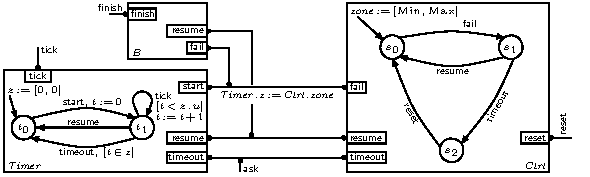
\includegraphics[width=\columnwidth]{BIPspec-ArchFailureTimerMax-v3}
  \caption{The BIP specification of the Failure Monitor architecture}
  \label{schema:ArchFailure:BIP}
\end{figure}

Figure~\ref{schema:ArchFailure:BIP} shows a refined version of the
Failure Monitor architecture used in~\cite{CubETH-case-study}.
Contrary to standard BIP models, architectures comprise one or several
\emph{operand} components, whereof only the set of \emph{ports} is
given.  Here, the operand component is $\NameOprnd$ and its interface
consists of the ports $\PortFinish$, $\PortResume$ and $\PortFail$.
The two \emph{coordinator} components\mdash $\NameCtrl$ and
$\NameTimer$\mdash are standard BIP components insofar as they also
have their \emph{behaviour} specified by finite automata extended with
local data variables.  Transitions of these automata are labelled with
the ports of the corresponding components, Boolean guards and update
functions on local variables.  For instance the loop transition
$\tstate{1} \goesto{\PortTick, \GuardTick[], \TimerUpd[]} \tstate{1}$
in the $\NameTimer$ component is labeled by the port $\PortTick$, it
can be fired only when the current value of the local variable $t$ is
greater than $0$.  Upon firing, this transition decrements the value
of $t$ by $1$.  When omitted, the default guard (\resp update
function) is the constant predicate $\true$ (\resp the $\mathit{skip}$
operator).  The constant $\mathrm{Max}$, in $\tstate{0}
\goesto{\PortStart, \TimerInit[]} \tstate{1}$, is a parameter of the
architecture.\noteLH{It looks like Max is in zone, I do not understand}

\noteLH{Ludo ou simon: essayer de remonter la description generique en debut de section}
Connectors are hierarchical, tree-like structures with component ports
at the leaves.  They define sets of \emph{interactions}, based on the
attributes of the connected ports~\cite{BliSif08-acp-tc}, which may be
either \emph{trigger} (triangles in Fig.~\ref{schema:ArchFailure:BIP})
or \emph{synchron} (bullets in Fig.~\ref{schema:ArchFailure:BIP}).
%
If all sub-connectors of a connector are synchrons, then an
interaction may be executed by the connector only if each subconnector
can contribute.
%
If at least one of the sub-connectors is a trigger, then any
interaction consisting of contributions of any set of sub-connectors,
\emph{involving at least one of the triggers}, can be executed.
%
For instance, the two ports $\NameTimer.\PortStart$ and
$\NameCtrl.\PortFail$ are always synchronised, since they belong to
the same binary sub-connector, where they are both synchrons.  In
particular, this means that whenever the transition $\cstate{0}
\goesto{\PortFail} \cstate{1}$ is fired, so is the transition
$\tstate{0} \goesto{\PortStart, \TimerInit[]} \tstate{1}$,
initialising the timer.  The binary connector $\NameTimer.\PortStart
\bullet\!\!\!-\!\!\!-\!\!\!\bullet \NameCtrl.\PortFail$ is a
sub-connector of a hierarchical connector, where the port
$\NameOprnd.\PortFail$ is a trigger.  Thus, the above interaction can
only happen together with $\NameOprnd.\PortFail$, forming a
ternary interaction.  On the contrary, being a trigger, the port
$\NameOprnd.\PortFail$ can fire alone, forming a singleton
interaction.  The composition semantics of BIP systems consists in
firing exactly one interaction, enabled through at least one of the
top-level connectors, at each execution round.

Finally, \emph{priorities}\mdash defined by a strict partial order on
the set of possible interactions\mdash narrow the choice among the
enabled interactions at any given round.  The default priority is the
so-called \emph{maximal progress}, whereby among any two interactions
$a \subset b$ (as sets of ports), $b$ has higher priority than $a$.
For example, the port $\NameOprnd.\PortFail$ will never fire alone in
a global state, where both $\NameTimer.\PortStart$ and
$\NameCtrl.\PortFail$ are enabled.
%
%% Adding priorities $\NameOprnd.\PortFinish < \NameCtrl.\PortReset$ and
%% $\NameOprnd.\PortFinish < \NameOprnd.\PortResume$, ensures that, after
%% a failure, the operation performed by $\NameOprnd$ cannot finish
%% unless it is explicitly resumed or the system is reset.

Application of the Failure Monitor architecture ensures that, whenever
a failure is registered in the operand component, the system will be
reset, unless a resumption is registered within $\mathrm{Max}$ time
units (more details in Sect.~\ref{section:resultOA}).

%****************************************************************
\subsection{Architectures}
\label{secn:archi}

\noteLHin{should we say that always epsilon C is the epsilon of C?}

\begin{definition}[Architecture]
  \label{defn:arch}
  An \emph{architecture} is a tuple $A = (\cC, V_A, P_A, \export[A], \Gamma)$,
  where $\cC$ is a finite set of \emph{coordinating components}
  with pairwise disjoint sets of ports and variables, such that
  $\bigcup_{C \in \cC} P_C \subseteq P_A$ and
  $\bigcup_{C \in \cC} V_C \subseteq V_A$;
%
  $\export[A] : P_A \rightarrow 2^{V_A}$ is an export function, such
  that $\export[A](p) = \export[C](p)$, for any $C \in \cC$ and $p \in
  P_C$ and $\export[A](p) \subseteq V_A \setminus \bigcup_{C \in \cC}
  V_C$ for any $p \in P_A \setminus \bigcup_{C \in \cC} P_C$; and
%
  $\Gamma \subseteq 2^{P_A} \times \guards{V_A} \times \exprs{V_A}$
  is an interaction model over \hl{$(V_A, P_A, \export[A])$}.
\end{definition}

\begin{definition}[Application of an architecture]
  \label{defn:arch:application}
  Let $A = (\cC, V_A, P_A, \export[A], \Gamma)$ be an architecture and let $\cB$
  be a set of components, such that
%
  \begin{align}
    \bigcup_{B \in \cB} V_B \cap \bigcup_{C \in \cC} V_C = \emptyset\,,
    &&
    V_A \subseteq V \bydef{=} \bigcup_{B \in \cB \cup \cC} V_B\,,
    \\
    \bigcup_{B \in \cB} P_B \cap \bigcup_{C \in \cC} P_C = \emptyset\,,
    &&
    P_A \subseteq P \bydef{=} \bigcup_{B \in \cB \cup \cC} P_B\,,
  \end{align}
%
  \hl{and $\export[A](p) = V_A \cap \export[B](p)$, for any $B \in \cB$
  and $p \in P_A \cap P_B$.}
%
  The \emph{application of the architecture $A$ to the set of
  components $\cB$} is the component $ A(\cB) \bydef{=}
  \mu\bigl((\IMextend{\Gamma}{P})(\cC \cup \cB)\bigr)$, where
%
  $\IMextend{\Gamma}{P}$ is the \emph{extension} of the interaction
  model $\Gamma$ to the set of ports $P$, \ie the interaction model
  over $(V, P, \export)$, with
  \[
  \export(p) = 
  \begin{cases}
    \export[C](p), & \text{for all } C \in \cC, p \in P_C,
    \\
    \export[B](p), & \text{for all } B \in \cB, p \in P_B,
  \end{cases}
  \]
  defined by\noteLH{looks like this also depends on Pa}
%
  \begin{equation}
    \label{eq:im:extension}
    \IMextend{\Gamma}{P} \bydef{=}
    \setdefb{
      (a \cup a', g, e)
    }{
      (a, g, e) \in \Gamma, a' \subseteq P \setminus P_A
    }
    ;
  \end{equation}
%
  $\mu$ is the maximal progress priority model.
\end{definition}

\todoSBin{Define equivalence $\arequiv$?}

An architecture $A$ enforces coordination constraints on the
components in $\cB$.  The interface \hl{$(V_A, P_A, \export[A])$} of an
architecture $A$ contains all ports of the coordinating
components $\cC$ and some additional ports, which must belong to
the components in $\cB$.  In the application $A(\cB)$, the ports
belonging to $P_A$ can only participate in the interactions
defined by the interaction model $\Gamma$ of $A$.  Ports which do
not belong to $P_A$ are not restricted and can participate in any
interaction.  In particular, they can join the interactions in
$\Gamma$ (see \eq{im:extension}).  If the interface of the
architecture covers all ports of the system, \ie $P = P_A$, we
have $P\setminus P_A = \emptyset$ and the only interactions
allowed in $A(\cB)$ are those belonging to $\Gamma$.  Notice also
that the restrictions imposed by \defn{arch:application} on the
set of operand components $\cB$ ensure that an interaction in
$\IMextend{\Gamma}{P}$ can only refer to variables of the
participating components.
%
Finally, the definition of $\IMextend{\Gamma}{P}$ requires that
an interaction from $\Gamma$ be involved in every interaction
belonging to $\IMextend{\Gamma}{P}$.  To allow the ports from $P
\setminus P_A$ to be fired independently in $A(\cB)$, one must
have $(\emptyset, \true, \noop) \in \Gamma$.  

\begin{definition}[Composition of architectures]
  \label{defn:arch:composition}
  Let $A_i = (\cC_i, V_{A_i}, P_{A_i}, \export[A_i], \Gamma_i)$, for $i = 1,2$,
  be two architectures.  The \emph{composition} of $A_1$ and
  $A_2$ is the architecture $A_1 \arcomp A_2 = (\cC_1 \cup \cC_2,
  V_{A_1} \cup V_{A_2}, P_{A_1} \cup P_{A_2}, \export[A_1] \cup \export[A_2], \Gamma)$, where
%
  \begin{equation}
    \label{eq:arch:composition}
    \Gamma = \setdefb{
      (a, g^1 \land g^2, e^1 \expmix e^2) 
    }{
      (a \cap P_{A_i}, g^i, e^i) \in \Gamma_i,
      \text{ for } i = 1,2
    }
    \,.
  \end{equation}
\end{definition}

\begin{proposition}[Properties of $\arcomp$]
  \label{prop:arcomp:nice}
  Architecture composition $\arcomp$ is commutative and
  associative; it is idempotent if all coordinating components
  are deterministic; $A_{id} = \bigl(\emptyset, \emptyset,
  \emptyset, \emptyset, \{(\emptyset, \true, \noop)\}\bigr)$ is its neutral element, \ie for
  any architecture $A$, we have $A \oplus A_{id} \arequiv A$.
  Furthermore, for any component $B$, we have $A_{id}(B) = \mu(B)$.
\end{proposition}
%
\begin{proof}[Sketch of the proof]
  Commutativity and associativity follow from the corresponding
  properties of set union, Boolean conjunction and
  \todoSB{Check ``semi''}\hl{semilattice meet}.
%
\todoLH{Check when equivalence is defined}
  Suppose we have two architectures $A \arequiv A'$.  This does not
  necessarily mean that their sets of coordinating components
  coincide.  However, if all the involved coordinating components
  are deterministic, then, in any state of $(A \arcomp A')(\cB)$,
  both architectures will impose the same restrictions, enabling
  the same interactions between the coordinating and operand
  components.  Hence, we have $(A \arcomp A')(\cB) = A(\cB) =
  A'(\cB)$.  Since this holds for any set of components $\cB$, we
  conclude that $A \arcomp A' \arequiv A \arequiv A'$.
%
  The properties of $A_{id}$ follow immediately from the
  definitions of architecture application and composition.
\end{proof}

The last statement of \prop{arcomp:nice} highlights a subtle point:
$A_{id}$ is the neutral element of the $\arcomp$ operator\mdash it is
not the identity operator on components.

%****************************************************************
\subsection{Preservation of safety properties}
\label{secn:safety}

For a component $B$, we denote $S_{\semopen{B}}$,
$s^0_{\semopen{B}}$ the corresponding constituents of
$\semopen{B}$.

\begin{definition}[Safety properties]
  \label{defn:property}
  Let $B$ be a component.  A \emph{safety property} (below,
  simply \emph{property}) of $B$ is a state predicate $\Phi:
  S_{\semopen{B}} \rightarrow \sB$, such that $\bigl((q,
  \val{}{}) \models \Phi\bigr) \land (\val[\primeit]{}{} \order
  \val{}{})$ implies $(q, \val[\primeit]{}{}) \models \Phi$,
  where we write $(q, \val{}{}) \models \Phi$ iff $\Phi(q,
  \val{}{}) = \true$.  A property $\Phi$ is \emph{initial} if
  $s^0_{\semopen{B}} \models \Phi$.
  %% \todoSB{Do we need this?}\hl{;
  %% it is \emph{reachable} iff there exists a possibly empty path
  %% $s^0_{\semopen{B}} \goesto{a^1, \val{1}{}} s^1 \goesto{a^2,
  %%   \val{2}{}} \cdots \goesto{a^n, \val{n}{}} s^n$, such that
  %% $s^n \models \Phi$}.
\end{definition}

\todoSB{Cite the original paper somewhere.}
The main idea of our approach is that an architecture enforces
its characteristic property on the set of its operand components.
From this point of view, the set of coordinating components is
not relevant, neither are their states.  Thus, to talk about
properties enforced by architectures, we consider properties on
the unrestricted composition of the operand components as
formalized by the following definition.

\begin{definition}[Enforcing properties]
  \label{defn:impose}
  Let $A = (\cC, P_A, V_A, \export[A], \Gamma)$ be an architecture; let $\cB$
  be a set of components and $\Phi$ an initial property of
  their parallel composition $A_{id}(\cB)$ (see
  \prop{arcomp:nice}).  We say that \emph{$A$ enforces $\Phi$ on
    $\cB$} iff, for every state $s = (s_c, s_b)$ reachable in
  $\semopen{A(\cB)}$, with 
  $s_c \in \prod_{C \in \cC} S_{\semopen{C}}$ and
  $s_b \in \prod_{B \in \cB} S_{\semopen{B}}$,
  we have $s_b \models \Phi$.
\end{definition}

According to the above definition, when we say that an
architecture enforces some property $\Phi$, it is implicitly
assumed that $\Phi$ is initial for the coordinated components.
Below, we omit mentioning this explicitly.

\begin{definition}[Upwards compatibility]
  \label{defn:up:compat}
  \todoSB{Summarise in English and move to the appendix}
%
  Consider two architectures $A_i = (\cC_i, V_{A_i}, P_{A_i},
  \export[A_i], \Gamma_i)$, for $i = 1,2$.
%
  We say that $A_1$ and $A_2$ are \emph{upwards compatible} iff, for
  any two interactions $(a_i, g_i, e_i) \in \Gamma_i$, such that $a_1
  \cap P_{A_2} = a_2 \cap P_{A_1}$ (\ie they agree on the common ports
  of the two architectures), we have 1)~for any interaction $(b_1,
  h_1, f_1) \in \Gamma_1$, such that $a_1 \varsubsetneq b_1$, there
  exists an interaction $(b_2, h_2, f_2) \in \Gamma_2$, such that $a_2
  \subseteq b_2$, $b_1 \cap P_{A_2} = b_2 \cap P_{A_1}$ and the 
  implication  
%
  \begin{multline*}
    \left(
    \exists (q^1_C)^{C \in \supp{b_1} \cap \cC_1}:
    \exists (q^2_C)^{C \in \supp{a_2} \cap \cC_2}:
    \bigwedge_{
      \begin{multlined}
        \scriptstyle
        C \in \supp{b_1} \cap \cC_1 \cap
        \\
        \scriptstyle
        \supp{a_2} \cap \cC_2
      \end{multlined}
    }
    q^1_C = q^2_C
    \ \land
    \right.
    \\
    \begin{aligned}
      \exists \bigl(q^1_C \goesto{b_1 \cap P_C, g^{b_1}_C, f^{b_1}_C}\bigr)^{C \in \supp{b_1} \cap \cC_1}:
      & \quad \left.
      h_1 \land \bigwedge_{C \in \supp{b_1} \cap \cC_1} g^{b_1}_C
      \ \land \right.
      \\
      \exists \bigl(q^1_C \goesto{a_1 \cap P_C, g^{a_1}_C, e^{b_1}_C}\bigr)^{C \in \supp{a_1} \cap \cC_1}:
      & \quad \left.
      g_1 \land \bigwedge_{C \in \supp{a_1} \cap \cC_1} g^{a_1}_C
      \ \land \right.
      \\
      \exists \bigl(q^2_C \goesto{a_2 \cap P_C, g^{a_2}_C, e^{a_2}_C}\bigr)^{C \in \supp{a_2} \cap \cC_2}:
      & \quad
      \left.
      g_2 \land \bigwedge_{C \in \supp{a_2} \cap \cC_2} g^{a_2}_C
      \right) \implies 
    \end{aligned}
  \end{multline*}
%
  \begin{multline*}
    \left(
    \exists (q^2_C)^{C \in (\supp{b_2}\setminus\supp{a_2}) \cap \cC_2}:
            {\color{white}\bigwedge_{C \in \cC_1}}\right. % Fake bigwedge to make the parenthesis the right size
            \\
            \left.
            \exists \bigl(q^2_C \goesto{b_2 \cap P_C, g^{b_2}_C, f^{b_2}_C}\bigr)^{C \in \supp{b_2} \cap \cC_2}:
            h_2 \land
            \bigwedge_{C \in \supp{b_2} \cap \cC_2} g^{b_2}_C
            \right)
  \end{multline*}
%  
  holds for all valuations $\val{}{1} : V_{A_1} \rightarrow \data$
  and $\val{}{2} : V_{A_2} \rightarrow \data$; and 2)~symmetrically
  for any interaction $(b_2, h_2, f_2) \in \Gamma_2$, such that $a_2
  \varsubsetneq b_2$.
\end{definition}

\begin{theorem}[Preserving enforced properties]
  \label{thm:combining}
  Let $\cB$ be a set of components; let $A_i = (\cC_i, V_{A_i},
  P_{A_i}, \export[A_i], \Gamma_i)$, for $i = 1,2$, be two upwards compatible architectures
  enforcing on $\cB$ the properties $\Phi_1$ and $\Phi_2$
  respectively.  The composition $A_1 \arcomp A_2$ enforces on
  $\cB$ the property $\Phi_1 \land \Phi_2$.
\end{theorem}

%****************************************************************
%****************************************************************

\section{Open pNets}
\label{secn:pNets}
\todoLHin{rewrite after uniformisation}
pNets are tree-like structures, where the leaves are either
\emph{parameterised labelled transition systems (pLTSs)}, expressing the
behaviour of basic processes, or \emph{holes}, used as placeholders
for unknown processes, of which we only specify the set of possible
actions, this set is named the \emph{sort}.
Nodes of the tree (pNet nodes) are synchronising artifacts, using a
set of \emph{synchronisation vectors} that express the possible
synchronisation between the parameterised actions of a subset of the
sub-trees.

\subsection{The (open) pNets Core Model}
\label{section:pNets}


A pLTS is a labelled transition system with variables. Variables can be
used to characterise a state, as part of actions, guards, and
assignments. Without loss of generality and to simplify the formalisation, we suppose 
here that 
variables are local to each 
state: each state has its set of variables disjoint from the others. Transmitting 
variable values from one state to the other can be done by explicit assignment. 
%Similarly, to simplify the management of variables and without loss of expressivity, we 
%suppose that transitions looping to the same state does not do assignments.
Note that we make no assumption on the finiteness of the set of states, nor
on the finite branching of the transition relation.

We first define the set of actions a pLTS can use, let $a$
range over action labels. Action terms are  of the form $\alpha=a((?x_i)^{i \in I}, 
\Expr_j^{j \in J})$, where $(?x_i)^{i \in I}$ are input variables, $\Expr_j^{j \in J})$ 
are expressions.

\begin{definition}[pLTS]
\label{pLTS}
A pLTS is a tuple
$\pLTS\triangleq\mylangle S,s_0, \to\myrangle$ where:
\begin{itemize}
\item[$\bullet$]
$S$ is a set of states, $\vars(s)$ denotes the set of associated variables;
\item[$\bullet$]
$s_0 \in S$ is the initial state;
%\item[$\bullet$]
 %Variables in
%$\iv(\alpha)$ are assigned by the action, other variables can be assigned
%by the additional assignments.
\item[$\bullet$] $\to \subseteq S \times L \times S$ is the transition relation and 
$L$ is the set of labels of the form
% SB: I removed a new paragraph here, ok?
$\langle \alpha,~g,~u\rangle$,
where $\alpha$ is a parameterised action, $\alpha \in\actions{\variables}$; 
$g\in\boolexprs{\variables}$ is a guard over variables of the source state and the 
action, and $u\in\assigns{\variables}$
assigns updated value for variables in the destination state. 
If 
$s \xrightarrow{\langle \alpha,~g,~u\rangle} s'\in \to $ then 
% REMOVED BECAUSE USELESS: $\iv(\alpha)\!\subseteq\! \vars(s')$, 
		$\vars(\alpha)\backslash \iv(\alpha)\!\subseteq\! \vars(s)$, 
		$\vars(g)\!\subseteq\! \vars(s)\cup\vars(\alpha)$, and
		$\vars(\codom(u))\!\subseteq\! \vars(s)\cup\vars(\alpha)\land 
		\vars(\dom(u))\!\in\!\vars(s')$. %,  and $s= s'\Rightarrow J=\emptyset$. 
		
\end{itemize}
\end{definition}
\noteLH{is dom and codom clear?}
\noteSB{Not sure: I understand, because I know what is meant, but this is not a canonical use, so should be explained. Will be solved if we roll back to \mbox{$(?x_i := e_i)^{i \in I}$} or \mbox{$\overline{?x := e}$}.}
Now we define
pNet nodes, as constructors for hierarchical behavioural structures.
A pNet has a set of sub-pNets that can be either pNets or pLTSs, and a
set of holes, playing the role of process parameters.

A composite pNet consists of a set of sub-pNets exposing
a set of actions, each of them synchronising actions in each of
the sub-pNets. The synchronisation between global actions and
internal actions is given by  \emph{synchronisation vectors}: a
synchronisation vector synchronises one or several internal actions, and
exposes a single resulting global action.
Actions involved at the pNet level (in the synchronisation vectors) do
not have input variables, \ie they 
have the form $a(\Expr_j^{j \in J})$.


\begin{definition}[pNets]\label{def-pnets}
A pNet is a hierarchical structure where leaves are pLTSs and holes\footnote{Typing can 
be added to pNets by defining and checking their interfaces, called 
sort~\cite{HMZ-FORTE2016}}:
$\pNet\triangleq \pLTS~|~\mylangle \pNet_i^{i\in I}, J, \symb{SV}_k^{k\in 
K}\myrangle$
where
\begin{itemize}
\item[$\bullet$] $\pNet_i^{i\in I}$ is the family of sub-pNets;
%  $\pNet_i^{i\in I}$ is a family of sub-pNets where $I\in\I_\P$ is the set over which 
%sub-pNets are indexed.

\item[$\bullet$] $J$ is a set of indexes, called \emph{holes}.
$I$ and $J$ are \emph{disjoint}: $I\!\cap\! J=\emptyset$,  $I\!\cup\! J\neq\emptyset$
%\item[$\bullet$] $\Sort_j \subseteq \AlgAS$ is a set of action terms, denoting the 
%\emph{sort} of
%hole $j$.

\item[$\bullet$] $\symb{SV}_k^{k\in K}$ is a set of
  synchronisation vectors. % (\hl{$K\in\I_\P$}). 
$\forall k\!\in\! K,
  \symb{SV}_k\!=\SV{\!\alpha_{l}^{l\in I_k \uplus J_k}}{\alpha'_k}{g_k}$, where
  $\alpha'_k\in \actions{\variables}$, $I_k\subseteq I$, $J_k\subseteq J$, and 
  $\vars(\alpha'_k)\subseteq \bigcup_{l\in I_k\uplus 
  J_k}{\vars({\alpha_l})}$. The global action of a vector $\symb{SV}_k$ is
$\alpha'_k$. The Boolean expression $g_k $, such that $\vars(g_k)\subseteq \bigcup_{l\in 
I_k\uplus J_k}{\vars({\alpha_l})}$, is a guard associated to the vector.


\end{itemize}
We define the set of holes and leaves of a pNet as follows:
  \begin{itemize}
\item
The set of holes $\Holes(\pNet_{i_1})$ of a pNet is the indexes of the holes of the pNet 
itself plus the indexes of all the holes of its subnets (we suppose those indexes 
disjoints).
%
%defined inductively; the sets of holes
%in a pNet node and its subnets are all disjoint:
%  \[\begin{array}{l}
%\Holes(\mylangle S,s_0, \to\myrangle) \!=\! \emptyset \\
%\Holes(\mylangle \pNet_i^{i\in I}\!,\Sort_j^{j\in J}\!, \overline{\symb{SV}}\myrangle) 
%=J\uplus{\displaystyle \bigcup_{i\in 
%I}\Holes(\pNet_i)}\\
%\forall i\in I.\, \Holes(\pNet_i)\cap J=\emptyset\\
%\forall i_1,i_2\in I.\,i_1\neq i_2\Rightarrow  
%\Holes(\pNet_{i_1})\cap\Holes(\pNet_{i_2})=\emptyset
%\end{array}\]
\item
The set of leaves of a pNet is the set of all pLTSs occurring in the structure, as an 
indexed family of the form $\Leaves(\pNet)= \mylangle \pNet_i \myrangle^{i \in L}$.
is said to be \emph{open}.
\end{itemize}
A pNet $Q$ is \emph{closed} if it has no hole: $\Holes(Q)=\emptyset$; else it
is said to be \emph{open}.
\end{definition}






\subsection{Operational Semantics for Open pNets}
\label{section:op-semantics}

\noteLH{a pred is a g a post is a e}
The semantics of open pNets will be defined  as an open automaton. An open
automaton is an automaton where each transition composes the actions of several holes, 
the transition occurs if some predicates hold, and can involve a 
set of state modifications.
%\TODO{adopt a uniform notation for open transitions, almost each instance has a 
%different 
%notation! I suggest p,l,pr,po using \{\} for p,l,po as they are sets}
\begin{definition}[Open transitions]
	\label{def:OpenTransitions}
	An \emph{open transition} over a
	set $J$ of holes  and a set of states $\mathcal{S}$ is 
	a structure of the form:	
	\begin{mathpar}
	\inferrule*[myfraction=\reddottedrule]
	{	\beta_j^{j\in J}, \Pred, \Post}
	{s \OTarrow {{\alpha}}s'}
	\end{mathpar}
	Where $s, s'\in\mathcal{S}$ and $\beta_j\in\actions{\variables}$
        is an action of the hole $j$. $v$ is a variable denoting the resulting action
        of this open transition. \Pred\ is a predicate 
	over the different variables of the
	terms, labels, and states  $\beta_j$, $s$, $\alpha$. $\Post\in 
	\assigns{\variables}$\ is 
	a set of assignments that are the effects of the transition.
Open transitions are identified modulo logical equivalence on their predicate.
\end{definition}
%\begin{definition}[Open transitions]
%	\label{def:OpenTransitions}
%	An \emph{open transition} over a set \noteSB{In the architecture section, I say that 
%we omit indices on $\goesto{}$ and that they are always clear from the 
%context.}\hl{$(S_i,s_{0 i}, \rightarrow_i)^{i\in
%	I}$} of LTSs, a
%	set $J$ of holes with sorts $\Sort_j^{j\in J}$, and a set of states $\mathcal{S}$ is 
%	a structure of the form:	
%	\begin{mathpar}
%	\inferrule*[myfraction=\reddottedrule]
%	{\{s_i~{\xrightarrow{a_i}}_i ~s_i^{\prime}\}^{i\in I},
%		\{\xrightarrow{b_j}_j\}^{j\in J}, \Pred, \Post}
%	{s \OTarrow {v}s'}
%	\end{mathpar}
%	Where $s, s'\in\mathcal{S}$ and for all
%        $i\in I$, $s_i{\xrightarrow{a_i}}_i s_i^{\prime}$ is a transition of the
%	LTS $(S_i,s_{0 i}, \rightarrow_i)$, and \noteSB{Why insist on ``transition'' and 
%$\goesto{b_j}_j$? Why not simply ``$b_j$ is an action in the sort 
%$\Sort_j$?}\hl{$\xrightarrow{b_j}_j$
%        is a transition of the hole $j$}, for any action $b_j$ in the
%        sort $\Sort_j$.  
%        of this open transition. \Pred\ is a predicate 
%	over the different variables of the
%	terms, labels, and states $s_i$, $b_j$, $s$, $v$. \Post\ is a set of equations that 
%	hold \emph{after the open transition}, they are represented as a substitution of the 
%	form $\{x_k\gets \Expr_k\}^{k\in K}$ \noteLH{considering the level of abstraction I 
%	would like to just put $\Post_=e$}
%	where $x_k$ are variables of $s'$, $s'_i$, and $e_k$ are expressions over the other 
%	variables of the open transition.
%\end{definition}


\begin{example}\emph{An open-transition.}
  \label{OT:enable-composed}
  The \texttt{EnableCompL} pNet of Fig. \ref{schema:enable-composed} has 2 controllers 
  and 2 holes. One of its possible open-transition is:

 \smallskip
 $  OT_2  = \openrule{ 
							(P\mapsto \delta(x4), Q\mapsto accept(x4))               
%                            \xrightarrow{\delta(x4)}_P ~~
%                            \xrightarrow{accept(x4)}_Q 
                      }
  %  {\ostate{00} \xrightarrow{\underline{\delta(x1)}} \ostate{10}}
    {A1_0 \OTarrow{\underline{\delta(x4)}} A1_1}
  $\noteSB{The underline notation did not appear until here.}
\end{example}

It is important to understand the difference between the red dotted rule and a normal 
inference rule. They correspond to two different logical levels.
 The open transition is itself a logical implication, but using a simple logic (with the 
 expressive power that is given to the predicate and necessary include logical 
 propositions and equality). We differentiate classical (black) inference rules that use 
 an expressive logic and are paper rules from open transition rules that use a simpler 
 logic, 
 will be embedded into automata transitions, and could typically be handled in a 
 mechanical way.


\begin{definition}[Open automaton]
	\label{def:open-automaton}
	An \emph{open automaton} is a structure\\ $A =
	<J,\mathcal{S},s_0,\mathcal{T}>$ where:
	\begin{itemize}
		\item[$\bullet$]   $J$ is a  set of indices,
		\item[$\bullet$]   $\mathcal{S}$ is a set of states and $s_0$ an initial state
		among $\mathcal{S}$,
		\item[$\bullet$] $\mathcal{T}$ is a set of open transitions and for each
		$t\in \mathcal{T}$ there exist  $J'$ with  $J'
		\subseteq J$, such that $t$ is an open transition over  $J'$,
		and  $\mathcal{S}$.
		
	\end{itemize}
\end{definition}
	

%
%Then the semantics of a pNet is characterized by a set of {\em open
%transitions}, where the hypotheses on process parameters are
%replaced by 1) transitions of the pLTSs at the leaves, and 2) formal
%hypotheses on the transitions of the holes. A {\em predicate} is used
%to relate the parameters and names appearing in the actions of the
%leaves and the holes involved in the rules, but also appearing in  the resulting action.

We define states of open pNets as tuples of states, where we denote tuples
in structured states as $\triangleleft\ldots\triangleright$ for distinguishing tuple 
states from other tuples.
\begin{definition}[States of open pNets]\label{def-states}
  A state of an open pNet is a tuple (not necessarily finite) of the
  states of its leaves.

  For any pNet p, let $\Leaves(p) = \mylangle S_i,{s_i}_0, \to_i\myrangle^{i \in L}$ be 
  the set of pLTS at its leaves,
  then $States(p) = \{\triangleleft s_i^{i\in L}
  \triangleright| \forall i\in L. s_i \in S_i\}$.
A pLTS being its own single leave:
  $States(\mylangle S,s_0, \to\myrangle) = \{\triangleleft s \triangleright| s \in S\}$.

The initial state is defined as:
$InitState(p) = \triangleleft {{s_i}_0}^{i\in L}  \triangleright$.
\end{definition}



%% \begin{example} \emph{State of a pNet}
%%   The states of pNet \texttt{EnableCompL} are:
%%   $\triangleleft 00 \triangleright, \triangleleft 10 \triangleright, \triangleleft 11 
%%\triangleright$
%% \end{example}

\paragraph{Predicates:}
Let
$\mylangle\overline{\pNet},\overline{\Sort},\overline{\symb{SV}}\myrangle$
be a pNet. Consider a synchronisation vector $\symb{SV}\in \overline{\symb{SV}}$. We 
define a
predicate $\Pred$ relating
the actions of the involved sub-pNets and the resulting actions. This predicate verifies:
\begin{multline}
\Pred_{\symb{sv}}(\SV{{(\alpha'_i)}^{i\in I}, {(\beta'_j)}^{j\in J}} 
{\alpha'} {g}, \alpha_i^{i\in I}, \beta_j^{j\in J}, \alpha)\Leftrightarrow \\
\forall i\in I.\, \alpha_i=\alpha'_i\land \forall j \in J.\, \beta_j=\beta'_j \land 
\alpha=\alpha' 
\land g
\end{multline}


 

Somehow, this predicate entails a verification of satisfiability in the sense that if the 
predicate $\Pred_{\symb{sv}}$ is not satisfiable, then the transition associated with the 
synchronisation will not occur in the considered state. 


In any other case (if the action families do not match or if there is no valuation of
variables such that the above formula can be ensured) the predicate is undefined.

This definition is not constructive but it is easy to build the predicate constructively
by brute-force unification of the sub-pNets
actions with the corresponding vector actions, possibly followed by a simplification
step.


We build the semantics of open pNets as an open automaton where LTSs are the pLTSs at
the leaves of the pNet structure, and the states are given by 
Definition~\ref{def-states}. The open transitions first
 project the global state into states of the leaves, then apply
pLTS transitions on these states, and compose them with the sort of the holes. %The pNet
%structure does not appear in the open-automaton, only the
%set of Holes and the set of Leaves.
The semantics    instantiates \emph{fresh} variables, additionally, for an action 
$\alpha$, $\fresh(\alpha)$ means all variables in $\alpha$ are fresh.


\begin{definition}[Operational semantics of open pNets]
	\label{def:operationalSemantics}
	The semantics of a pNet $p$ is an open automaton $A = 
	<Holes(p),States(p),InitState(p),
	\mathcal{T}>$ where $\mathcal{T}$ is the smallest set of open transitions		
	satisfying the rules below:
%	\begin{itemize}
%		\item $J$ is the set of holes: $Holes(p)= J$. 
		%  \item $\overline{L}^L = Leaves(p), \overline{H}^J = Holes(p)$
%		\item ${\mathcal{S}} = States(p)$ and $s_0 = InitState(p)$
%		\item $\mathcal{T}$ is the smallest set of open transitions		satisfying the 
%rules below:
%	\end{itemize}
	
	%% \TODO{ We should be careful here: after (re) reading "Huimin
	%% 	Lin, 'Symbolic Transition Systems with Assignements', Concur'96" I
	%% 	think handling assignments is not trivial, even for comparisons of pLTSs. }


	
	The rule for a pLTS  checks that the guard 
	is verified and transforms assignments into post-conditions:
	
	\begin{description}
		\item[{\bf Tr1:}]
	$\inferrule
		{ s \xrightarrow{\langle \alpha,~g,~u\rangle} s'\in \to  }
		{ \mylangle  S,s_0, \to \myrangle
			\models
			\openrule
			{\emptyset ,
			g,u}
			{\ostate{s} \OTarrow{\alpha} \ostate{s'}}
		}
		$
	\end{description}
%	Note that this note is greatly simplified by the fact that variables are local to 
%	thread; introducing global state variables or accepting loops to the same 
%	state would 
%	require to reason 
%	on the scope of 
%	each variables, and to introduce additional variables to handle the several occurence 
%	of the same pLTS variable in the predicates. Indeed the constraints on pLTS 
%	transitions 
%	ensure that the same variable never appears both on the left and on the right of the 
%	equations of a predicate.
	
	The second rule deals with pNet nodes: for each possible
	synchronisation vector (of index $k$) applicable to the rule subject, the premisses
	include one {\em open transition} for each sub-pNet involved , one possible
	{\em action} for each Hole involved, and the predicate relating these
	with the resulting action of the vector. The sub-pNets involved are split between two 
	sets, $I_2$ for subnets that are pLTSs, and $I_1$ for the others, $J$ is the set of 
	holes involved in the transition\footnote{Formally, if $SV_k \!=\! \SV{\alpha_m^{m 
	\in M}}{\alpha'}{g}$ is a synchronisation vector  of \pNet\  then $J=M\cap 
	\Holes(\pNet)$, $I_2=M\cap \Leaves(\pNet)$,  $I_1=M\setminus J \setminus 
	I_2$}.                                                                    
	           
	                                                       
	\begin{description}
		\item[{\bf Tr2:}]
	\end{description}
	
	\noindent
\begin{mathpar}
    \mprset {vskip=1ex}
\inferrule
    {
\Leaves(\mylangle \overline{\pNet}, \overline{\Sort}, \symb{SV}_k^{k\in 
    	K}\myrangle) \!=\! \pLTS_l^{l\in L} \qquad  	
k\!\in\! K \qquad SV_k \!=\! \SV{(\alpha'_m)^{m \in I_1\uplus I_2\uplus J}}{\alpha'}{g} 
\\
\\     	
	\forall m\!\!\in\!\! I_1. {\pNet_m 
	\models\openrule
    	{
    	\beta_{j}^{j\in J_m}, \Pred_m, \Post_m}
    	{\ostate{s_{i}^{i \in L_m}} \OTarrow {\alpha_m}
    		\ostate{(s_i^\prime)^{i\in L_m}}} }	
  \qquad
\forall m\!\!\in\!\! I_2.		{ \pNet_m 
    	 \models
    	\openrule
    	{\emptyset, \Pred_m, \Post_m}
    	{\ostate{s_m} \OTarrow {\alpha_m}
    		\ostate{s_m'}} }\\\\
     J' = \biguplus_{m\in I_1}\!\! J_m \uplus J 	\\
    	\Pred = \bigwedge_{m\in (I_1\uplus I_2)}\!\! \Pred_m \land
    	\Pred_{\symb{sv}}(SV_k,\alpha_m^{m\in (I_1\uplus I_2)},\beta_j^{j\in J},\alpha)\\ 
    		I' = \biguplus_{m\in I_1}\!\! I_m \uplus I_2
    	\\\forall i\in	L\backslash I'.\,s'_i=s_i \\
    \fresh(\alpha'_m,\alpha',\beta_j,\alpha) 
    }
    {\mylangle \overline{\pNet}, \overline{\Sort}, \symb{SV}_k^{k\in K}\myrangle
    	\models
    	{\openrule
    		{
    		{\beta_j}^{j\in J^\prime}, \Pred, \uplus_{m\in I_1\uplus I_2} 
    		\Post_m}
    		{\ostate{s_i^{i\in L}} \OTarrow {\alpha}
    			\ostate{(s_i^\prime)^{i\in L}}}
    	}
    }
\end{mathpar}      

%OLD	\begin{description}
%		\item[{\bf Tr2:}]\noteSB{I do not understand why the second line $pNet_m 
%\models\dots$ is not subsumed by the first one?}
%	\end{description}
%	
%	\noindent
%    $\inferrule
%    {k\!\in\! K \\SV_k \!=\! \alpha_m^{m \in I\uplus J} \!\to\! 
%    \alpha' |g \\
%    	Leaves(\mylangle \pNet_i^{i\in I'}, \overline{\Sort}, \symb{SV}_k^{k\in 
%    	K}\myrangle) \!=\! \pLTS_l^{l\in L} \\    	
%    	\forall m\!\!\in\!\! I. 	
%    {\left(\begin{array}{l}
%	{\pNet_m \models\inferrule*[myfraction=\reddottedrule]
%    	{\{s_{i}\xrightarrow{a_{i}}_i s_{i}'\}^{i\in I_m^\prime},
%    	\{\xrightarrow{b_{j}}_j\}^{j\in J'_m}, \Pred_m, \Post_m}
%    	{\ostate{s_{i}^{i \in L_m}} \OTarrow {v_m}
%    		\ostate{(s_i^\prime)^{i\in L_m}}}\lor }\\
%		{ \pNet_m 
%    	 \models
%    	\inferrule*[myfraction=\reddottedrule]
%    	{\{s_m \xrightarrow{v_m} s_m'\},\emptyset, \Pred_m, \Post_m}
%    	{\ostate{s_m} \OTarrow {v_m}
%    		\ostate{s_m'}} \land I'_m=\{m\} \land J'_m=\emptyset}
%\end{array}\right)}\\
%    	%\land
%    	%Leaves(\pNet_m) = \overline{\pLTS}^{L_k})  	
%     J' = \biguplus_{m\in I}\!\! J'_m \uplus J 	\\
%    	\Pred = \bigwedge_{m\in I}\!\! \Pred_m \land
%    	\Pred_{\symb{sv}}(SV_k,v_m^{m\in I},b_j^{j\in J},v)\\ 
%    		I' = \biguplus_{m\in I}\!\! I_m'
%    	\\\forall i\in	L\backslash I'.\,s'_i=s_i \\
%    {\tt fresh}(\alpha_m,\alpha',b_j,v) 
%    }
%    {\mylangle \pNet_i^{i\in I'}, \overline{\Sort}, \symb{SV}_k^{k\in K}\myrangle
%    	\models
%    	{\inferrule*[myfraction=\reddottedrule]
%    		{\{s_i\xrightarrow{a_i}_i s_i^{\prime}\}^{i\in I^\prime},
%    		\{\xrightarrow{b_j}_j\}^{j\in J^\prime}, \Pred, \uplus_{m\in I_k} 
%    		\Post_m}
%    		{\ostate{s_i^{i\in L}} \OTarrow {v}
%    			\ostate{(s_i^\prime)^{i\in L}}}
%    	}
%    }
%    $
	\medskip
%        \TODO{may be explain how $\Pred(SV,a_i^{i\in I_k},b_j^{j\in
%            J_k},v)$ is built ? You mean more than what is written on previous page????}
	%%    \TODO{I have tentatively added the sort constraint on hole actions, that was
	%%not included in the first version... I'm unsure whether this is the best place to
	%%include it, because it may change the decidability conditions on predicates}
	
\end{definition}


%****************************************************************
%****************************************************************

\section{Encoding of architectures into open pNets}
\label{secn:encoding}

%****************************************************************
%****************************************************************

\section{SMT encoding of open pNets}
\label{secn:smt}

%****************************************************************
%****************************************************************

\section{Case study}
\label{secn:case-study}

\begin{figure}[t]
  \centering
  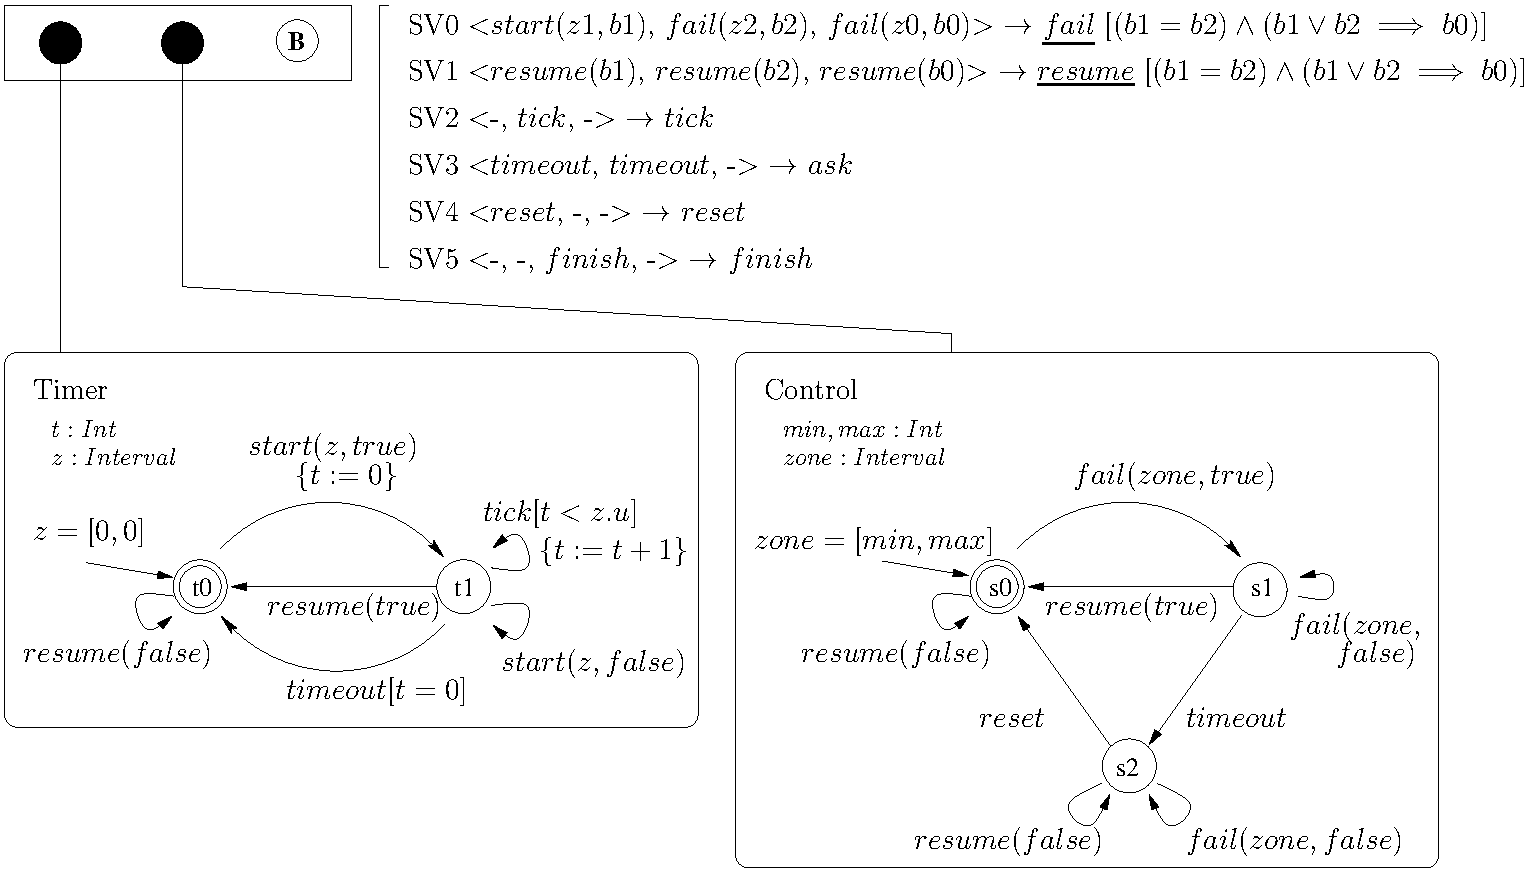
\includegraphics[width=\columnwidth]{FailureTimerZonePNET}
  \caption{The pNET encoding the Failure Monitor architecture}
  \label{schema:ArchFailure:BIP}
\end{figure}


%****************************************************************
%****************************************************************

\section{Related work}
\label{secn:related}

%****************************************************************
%****************************************************************

\section{Conclusion}
\label{secn:conclusion}

%****************************************************************
%****************************************************************

\bibliographystyle{abbrv}
\bibliography{biblio}

%****************************************************************
%****************************************************************
\appendix
\clearpage

\section{Proofs}

\begin{lemma}
  \label{lem:onlyone}
  Let $A = (\cC, V_A, P_A, \export[A], \Gamma)$ be an architecture and denote
  by $\Gamma_\cC \bydef{=}
%
  \setdef{
    (a \cap P_\cC, \true, \noop)
  }{
    (a, g, e) \in \Gamma
  }$, with $P_\cC = \bigcup_{C \in \cC} P_C$,
%  
  the projection of $\Gamma$ onto the coordinating components of
  $A$.  Consider the architecture $A' = (\{C'\}, V_A, P_A, \export[A],
  \Gamma)$, where $C' = \Gamma_\cC(\cC)$.  For any set of
  components $\cB$, satisfying the conditions of
  \defn{arch:application}, we have
  $\semopen{A(\cB)} = \semopen{A'(\cB)}$.
\end{lemma}
%
\begin{proof}
  First of all, notice that, by \defn{im:sem},
  $V_{C'} = \bigcup_{C \in \cC} V_C$ and $P_{C'} = P_\cC = \bigcup_{C \in \cC} P_C$.
  The conditions of \defn{arch} are satisfied and $A'$ is indeed
  an architecture.  Furthermore, $\cB$ satisfies the conditions
  of \defn{arch:application} \wrt $A'$.  Hence, the component
  $A'(\cB)$ is well defined.

  Clearly the state spaces and initial states %% and interfaces
  of both LTSs $\semopen{A(\cB)}$ and $\semopen{A'(\cB)}$
  coincide.  Thus, we only have to prove that so do the
  transition relations.  Let us assume that
  $\cC = C_i^{i \in I}$ and $\cB = B_j^{j \in J}$.
  We will use $q_i, q_i'$ to denote the states of
  $C_i$ and $q_j, q_j'$ to denote the states of $B_j$,
  and similarly for the valuations of variables.

  By \defn{comp:semantics},
%
  \begin{equation}
    \label{eq:lem1:trans:sem}
    (q_i, \val{}{i})^{i \in I} (q_j, \val{}{j})^{j \in J}
    \goesto{a, \val[\tilde]{}{}}
    (q_i', \val{\prime}{i})^{i \in I}
    (q_j', \val{\prime}{j})^{j \in J}
  \end{equation}
%  
  is a transition in $\semopen{A(\cB)}$ (\resp
  $\semopen{A'(\cB)}$) iff
%
  \begin{equation}
    \label{eq:lem1:trans}
    q_i^{i \in I} q_j^{j \in J}
    \goesto{a, g', e'}
    (q_i')^{i \in I} (q_j')^{j \in J}
    \,,
  \end{equation}
%
  is a transition in $A(\cB)$ (\resp $A'(\cB)$) and
%
  \begin{mathpar}
    \val{i \in I}{i} \val{j \in J}{j}
    \models g'
    \,,
    \and
    (\val{\prime}{i})^{i \in I} (\val{\prime}{j})^{j \in J}
    = \val[\tilde]{}{}[e']
    \,,
    \and
    \valdiff{\val{i \in I}{i} \val{j \in J}{j}}{
      \val[\tilde]{}{}} \subseteq \export(a)       
  \end{mathpar}
%
  (with $\export$ defined as in \defn{arch:application}).

  By \defn{im:sem} and \defn{priority:sem}, \eq{lem1:trans} is a transition in $A(\cB)$
  iff $a \neq \emptyset$, $(a, g, e) \in \IMextend{\Gamma}{P}$,
  where $P = \bigcup_{B \in \cB \cup \cC} P_B$, and
  %
  \begin{enumerate}
  \item\label{ab:start} for $i \in I$,\\
    $a \cap P_{C_i} \neq \emptyset$ and
    $q_i \goesto{a \cap P_{C_i},\, g_{C_i},\, e_{C_i}} q_i'$
    is a transition in $C_i$, or\\
    $a \cap P_{C_i} = \emptyset$ and $q_i = q_i'$
    (for covenience, we put $g_{C_i} = \true$ and $e_{C_i} = \noop$ in item~\ref{aux1} below);
  \item for $j \in J$,\\
    $a \cap P_{B_j} \neq \emptyset$ and
    $q_j \goesto{a \cap P_{B_j},\, g_{B_j},\, e_{B_j}} q_j'$
    is a transition in $B_j$, or\\
    $a \cap P_{B_j} = \emptyset$ and $q_j = q_j'$
    (for covenience, we put $g_{B_j} = \true$ and $e_{B_j} = \noop$ in item~\ref{aux1} below);
  \item\label{ab:end}\label{aux1} $g' = g \land \bigwedge_{i \in I} g_{C_i} \land
    \bigwedge_{j \in J} g_{B_j} \land \varphi_\mu$ and
    $e' = e; e_{C_i}^{i \in I}, e_{B_j}^{j \in J}$, where    
%
    \begin{equation}
      \label{eq:only1:maxprog:guard}
      \varphi_\mu = \bigwedge_{
        \begin{array}{c}
          q_i^{i \in I} q_j^{j \in J} \goesto{b, h, f} \text{ in }
          (\IMextend{\Gamma}{P})(\cC \cup \cB)
          \\
          a \varsubsetneq b
        \end{array}
      } \lnot h
      \,.
    \end{equation}
%
  \breakenumistart

  Similarly, \eq{lem1:trans} is a transition in
  $A'(\cB)$ iff $a \neq \emptyset$,
  $(a, g, e) \in \IMextend{\Gamma}{P}$ and
%
  \breakenumiend
% 
  \item \label{a1b:start} \label{only1:coord}
    $a \cap P_{C'} \neq \emptyset$ and 
    $(q_i)^{i \in I} \goesto{a \cap P_{C'}, g_{C'}, e_{C'}} (q_i')^{i \in I}$
    is a transition in $C'$, or\\
    $a \cap P_{C'} = \emptyset$ and $q_i = q_i'$,
    for all $i \in [1,m]$
    (for covenience, we put $g_{C'} = \true$ and $e_{C'} = \noop$ in
    item~\ref{aux2} below);
  \item for $j \in J$,\\
    $a \cap P_{B_j} \neq \emptyset$ and
    $q_j \goesto{a \cap P_{B_j}, g_{B_j}, e_{B_j}} q_j'$
    is a transition in $B_j$, or\\
    $a \cap P_{B_j} = \emptyset$ and $q_j = q_j'$
    (for covenience, we put $g_{B_j} = \true$ and $e_{B_j} = \noop$ in
    item~\ref{aux2} below);
  \item\label{aux2} $g' = g \land g_{C'} \land
    \bigwedge_{j \in J} g_{B_j} \land \varphi_\mu'$ and
    $e' = e; e_{C'}, e_{B_j}^{j \in J}$ (with $\varphi_\mu'$ defined as
    in \eq{only1:maxprog:guard}, but substituting $\{C'\}$ instead of $\cC$).
%
  \breakenumistart
  Notice that, for any $i \in I$, since
  $P_{C_i} \subseteq P_{C'}$, we have
  $a \cap P_{C_i} = (a \cap P_{C'}) \cap P_{C_i}$.
  Thus, if $a \cap P_{C'} \neq \emptyset$, 
  the transition in condition~\ref{only1:coord} above is
  present in $C'$ iff
  $(a \cap P_{C'}, \true, \noop) \in \Gamma_\cC$ and
  \breakenumiend
% 
  \item for $i \in I$,\\
    $a \cap P_{C_i} \neq \emptyset$ and
    $q_i \goesto{a \cap P_{C_i}, g_{C_i}, e_{C_i}} q_i'$
    is a transition in $C_i$, or\\
    $a \cap P_{C_i} = \emptyset$ and $q_i = q_i'$,
    (for covenience, we put $g_{C_i} = \true$ and $e_{C_i} = \noop$ in
    item~\ref{aux3} below);
  \item \label{a1b:end} \label{aux3} $g_{C'} = \bigwedge_{i \in I} g_{C_i}$ and
    $e_{C'} = e_{C_i}^{i \in I}$.
  \end{enumerate}

  Consider $(a,g,e) \in \IMextend{\Gamma}{P}$.  By
  \eq{im:extension}, this is equivalent to
  $(a \cap P_A, g, e) \in \Gamma$.
  Since $P_{C'} = P_\cC \subseteq P_A$, we have
  $a \cap P_{C'} = a \cap P_\cC = (a \cap P_A) \cap P_\cC$.
  Hence, by the definition of $\Gamma_\cC$ in the lemma statement,
  this is also equivalent to
  $(a \cap P_{C'}, \true, \noop) \in \Gamma_\cC$.

  Thus, conditions \ref{ab:start}\ndash\ref{ab:end} are satisfied iff
  so are conditions \ref{a1b:start}\ndash\ref{a1b:end} (to see that
  $\varphi_\mu$ is satisfied iff so is $\varphi_\mu'$, one has to
  consider the same two sets of conditions, but this time without the
  additional conjuncts $\varphi_\mu$ and $\varphi_\mu'$ in
  items~\ref{aux1} and \ref{aux2}, since no priority model is applied
  to obtain $C'$).  This proves that the transition relations of
  $\semopen{A(\cB)}$ and $\semopen{A'(\cB)}$ coincide and, therefore,
  $\semopen{A(\cB)} = \semopen{A'(\cB)}$.
\end{proof}

\begin{note}
  \label{rem:upwards:compat}
  Notice that, since, in the statement of \lem{onlyone}, 
  %
  \begin{enumerate}
  \item the interaction models are the same for both $A$ and $A'$, and
  \item $P_{C'} = P_\cC$,
  \end{enumerate}
  %
  substituting $A'$ for $A$ preserves upwards compatibility, \ie for any
  architecture $A''$, holds the following statement: $A$ and $A''$ are
  upwards compatible if and only if so are $A'$ and $A''$.
\end{note}

\begin{lemma}
  \label{lem:onestep}
  Let $\cB$ be a set of components; let $A_i = (\{C_i\}, V_{A_i},
  P_{A_i}, \export[A_i], \Gamma_i)$, for $i = 1,2$, be two upwards compatible architectures
  with one coordinator each, applicable to $\cB$.  Denote
  $P_i = P_{C_i} \cup \bigcup_{B \in \cB} P_B$.
  Finally, let
%
  $
  s_1 s_2 s
%
  \goesto{a, \tilde{\val{}{}}}
%
  s_1' s_2' s'
  $,
%
  be a transition in $\semopen{(A_1 \arcomp A_2)(\cB)}$, with
  $a \neq \emptyset$, 
  $s, s' \in \prod_{B \in \cB} S_{\semopen{B}}$
  and
  $s_i, s_i' \in S_{\semopen{C_i}}$ ($i=1,2$).
%
  Then, for $i=1,2$, either $a \cap P_i = \emptyset$ and $s_i s=
  s_i' s'$, or there exists a transition
%
  $
  s_i s
%
  \goesto{a \cap P_i, \val[\doubletilde]{}{}}
%
  s_i' s''
  $ 
%
  in $\semopen{A_i(\cB)}$, with
  $\val[\doubletilde]{}{}$ being the restriction of
  $\val[\tilde]{}{}$ to
  $V_i = V_{C_i} \cup \bigcup_{B \in \cB} V_B$ and
  $s' \order s''$.
\end{lemma}
%
\begin{proof}
  By \defn{comp:semantics}, every semantic state consists of a
  component state and a valuation of component variables.  Thus,
  we can expand $s_1 s_2 s \goesto{a, \tilde{\val{}{}}} s_1' s_2' s'$
  as
%
  \[
  (q_1, \val{}{1}, q_2, \val{}{2}, q, \val{}{})
%
  \goesto{a, \tilde{\val{}{}}}
%
  (q_1', \val[\primeit]{}{1}, q_2', \val[\primeit]{}{1}, q', \val[\primeit]{}{})
  \,.
  \]
%
  By \eq{im:sem} and \eq{priority:sem}, this implies
  that
  $(q_1, q_2, q) \goesto {a, g', e'} (q_1', q_2', q')$
  is a transition in $(A_1 \arcomp A_2)(\cB)$, with
%
  $g' = g \land g_1 \land g_2 \land g_\cB \land \varphi_\mu$
  and
  $e' = e; (e_1, e_2, e_\cB)$,
  where $(a, g, e) \in \Gamma$ (see \eq{arch:composition} for the
  definition of $\Gamma$);
%  
  $g_1$, $g_2$ and $e_1$, $e_2$ are, respectively, the guards and
  update expressions of the underlying transitions in the coordinating
  components $C_1$ and $C_2$;
%    
  \begin{mathpar}
    g_\cB = \bigwedge_{B \in \supp{a} \cap \cB} g_B
    \,,
    \and
    e_\cB = e_B^{B \in \supp{a} \cap \cB}
    \,,
  \end{mathpar}
%
  are the compositions of, respectively, the guards and update
  expressions of the operand components;
%    
  \begin{equation}
    \label{eq:onestep:maxprog:guard}
    \varphi_\mu = \bigwedge_{
      \begin{array}{c}
        (q_1, q_2, q) \goesto{b, h', f'} \text{ in }
        \bigl(\IMextend{\Gamma}{(P_1 \cup P_2)}\bigr)
        \bigl(\{C_1, C_2\} \cup \cB\bigr)
        \\
        a \varsubsetneq b
      \end{array}
    } \lnot h'
  \end{equation}
%
  is the conjunct encoding the maximal progress priority
  \eq{priority:sem}.  As above for $g'$, for each $(b, h', f')$ in
  \eq{onestep:maxprog:guard}, $h'$ can be decomposed as $h' = h \land
  h_1 \land h_2 \land h_\cB$ (without the maximal progress conjunct,
  since no priority is applied in $\bigl(\IMextend{\Gamma}{(P_1 \cup
    P_2)}\bigr)\bigl(\{C_1, C_2\} \cup \cB\bigr)$).
  
  By \eq{comp:semantics}, we also have
%
  \begin{align}
    \label{eq:guard}
    (\val{}{1}, \val{}{2}, \val{}{}) &\models g'
    \,,
    \\
    \label{eq:substitution}
    (\val[\primeit]{}{1}, \val[\primeit]{}{2}, \val[\primeit]{}{})
    &= \val[\tilde]{}{}[e']
    \,,
    \\
    \label{eq:transient}
    \valdiff{(\val{}{1}, \val{}{2}, \val{}{})}{\val[\tilde]{}{}}
    &\subseteq \export(a)
    \,.
  \end{align}
%
  If $a \cap P_1 = \emptyset$, then $\supp{a} = \{C_2\}$ and, by
  \eq{transient} and \defn{im:sem}, $s_1 = s_1'$ and $s = s'$
  (recall, \defn{im}, that, for $(a,g,e) \in \Gamma$, we have $e
  \in \exprs{V_a}$).  Hereafter, assume $a \cap P_1 \neq
  \emptyset$.

  By \eq{arch:composition}, for $i=1,2$, there exist $(a \cap P_{A_i},
  g^i, e^i) \in \Gamma_i$, such that $g = g^1 \land g^2$ and $e = e^1
  \land e^2$.
  %% Similarly, for each $(b, h', f')$ in \eq{onestep:maxprog:guard},
  %% there exist $(b \cap P_{A_i}, h^i, f^i) \in \Gamma_i$, such that
  %% $h = h^1 \land h^2$ and $f = f^1 \land f^2$.
%
  We want to show that the interaction $(a \cap P_1, g^1, e^1)$ is
  enabled in the state $(q_1, \val{}{1}, q, \val{}{})$ of
  $\semopen{A_1(\cB)}$.  To this end, we proceed in two steps:
%
  \begin{enumerate}
  \item \label{onestep:proof:im} We show that $(a \cap P_1, g^1,
    e^1)$ is enabled in the state $(q_1, \val{}{i}, q, \val{}{})$ of
    $\semopen{(\IMextend{\Gamma_1}{P_1})(\cB)}$.
  \item \label{onestep:proof:maxp} We show that $(a \cap P_1, g^1,
    e^1)$ is not inhibited in $\semopen{A_1(\cB)} =
    \semopen{\mu\bigl((\IMextend{\Gamma_1}{P_1})(\cB)\bigr)}$ by the
    maximal progress priority.
  \end{enumerate}

  \paragraph*{Step \ref{onestep:proof:im}}
  %% Denoting $P_\cB = \bigcup_{B \in \supp{a} \cap \cB} P_B$, 
  By \eq{im:sem}, we have
%
  \begin{mathpar}
    q_1 \goesto{a \cap P_{C_1}, g_1, e_1} q_1'
    \and
    \text{and}
    \and
    q_B \goesto{a \cap P_B, g_B, e_B} q_B',
    \text{ for each }
    B \in \cB
    \,.
  \end{mathpar}

  By \eq{guard}, we have
  $(\val{}{1}, \val{}{}) \models g^1 \land g_1 \land g_\cB$.

  Denoting \todoSB{One tilde is enough}$\val[\doubletilde]{}{1}$ the restriction of
%
  $\val[\tilde]{}{}$ to
  $V_1 = V_{C_1} \cup \bigcup_{B \in \cB} V_B$,
%
  we have, by \eq{substitution} and the monotonicity of
  expressions,
%
  $(\val[\primeit]{}{1}, \val[\primeit]{}{}) \order
  \val[\doubletilde]{}{1}[e^1; (e_1, e_b)]$.  \todoSB{Remove this}\hl{Notice that all
  variables affected by both $e^1$ and $e^2$ must necessarily
  belong to $\bigcup_{B \in \cB} V_B$.}  Hence,
%
  $\val[\doubletilde]{}{1}[e^1; (e_1, e_b)] =
  (\val[\primeit]{}{1}, \val[\doubleprimeit]{}{})$ with 
  $\val[\primeit]{}{} \order \val[\doubleprimeit]{}{}$.

  By \eq{comp:semantics} and \eq{im:sem}, we have
  $
  (q_1, \val{}{1}, q, \val{}{})
  \goesto{a \cap P_1, \val[\doubletilde]{}{1}}
  (q_1', \val[\primeit]{}{1}, q, \val[\doubleprimeit]{}{})
  $ in $\semopen{(\IMextend{\Gamma_1}{P_1})(\cB)}$.

  Symmetrically, we have 
  $
  (q_2, \val{}{2}, q, \val{}{})
  \goesto{a \cap P_2, \val[\doubletilde]{}{2}}
  (q_2', \val[\primeit]{}{2}, q, \val[\doubleprimeit]{}{})
  $ in $\semopen{(\IMextend{\Gamma_2}{P_2})(\cB)}$.   
   
  \paragraph*{Step \ref{onestep:proof:maxp}}
  Suppose that $a \cap P_1 \varsubsetneq b_1$, for some interaction
  $(b_1, h^1, f^1) \in \IMextend{\Gamma_1}{P_1}$ enabled in $(q_1,
  \val{}{1}, q, \val{}{})$.  Then, by upwards compatibility of $A_1$
  and $A_2$, there exists $(b_2, h^2, f^2) \in
  \IMextend{\Gamma_2}{P_2}$, enabled in $(q_2, \val{}{2}, q,
  \val{}{})$, such that $a \cap P_2 \subseteq b_2$ and $b_2 \cap P_1 =
  b_1 \cap P_2$.  By \eq{im:extension}, we have $(b_1 \cap P_{A_1},
  h^1, e^1) \in \Gamma^1$.  Furthermore,
%
  \begin{multline*}
    ((b_1 \cap P_{A_1}) \cup (b_2 \cap P_{A_2}))  \cap P_{A_1} =
    (b_1 \cap P_{A_1}) \cup (b_2 \cap P_{A_1} \cap P_{A_2}) =\\
    (b_1 \cap P_{A_1}) \cup ((b_2 \cap P_1) \cap P_{A_1} \cap P_{A_2}) =  
    (b_1 \cap P_{A_1}) \cup ((b_1 \cap P_2) \cap P_{A_1} \cap P_{A_2}) =\\
    (b_1 \cup (b_1 \cap P_2 \cap P_{A_2})) \cap P_{A_1} =
    b_1 \cap P_{A_1} 
  \end{multline*}
%
  Symmetrically, $(b_2 \cap P_{A_2}, h^2, e^2) \in \Gamma^2$ and
  $((b_1 \cap P_{A_1}) \cup (b_2 \cap P_{A_2})) \cap P_{A_2} = b_2
  \cap P_{A_2}$.  By \eq{arch:composition}, we then have $((b_1 \cap
  P_{A_1}) \cup (b_2 \cap P_{A_2}), h^1 \land h^2, f^1 \expmix f^2)
  \in \Gamma$ and, by \eq{im:extension}, $(b_1 \cup b_2, h^1 \land
  h^2, f^1 \expmix f^2) \in \IMextend{\Gamma}{(P_1 \cup P_2)}$.
%
  Since both $(b_i, h^i, f^i) \in \IMextend{\Gamma_i}{P_i}$ are
  enabled in the respective states $(q_i, \val{}{i}, q, \val{}{})$, we
  conclude that $(b_1 \cup b_2, h^1 \land h^2, f^1 \expmix f^2)$ is
  enabled in $(q_1, \val{}{1}, q_2, \val{}{2}, q, \val{}{})$.

  Since $a \cap P_1 \varsubsetneq b_1$ and $a \cap P_2 \subseteq b_2$,
  we have $a \varsubsetneq b_1 \cup b_2$.  Thus, $(b_1 \cup b_2, h^1
  \land h^2, f^1 \expmix f^2)$ contribute to $\varphi_\mu$ in
  \eq{onestep:maxprog:guard}.  Since $(b_1 \cup b_2, h^1 \land h^2,
  f^1 \expmix f^2)$ is enabled in $(q_1, \val{}{1}, q_2, \val{}{2}, q,
  \val{}{})$, we have $(\val{}{1}, \val{}{2}, \val{}{}) \models h^1
  \land h^2$ and, therefore $(\val{}{1}, \val{}{2}, \val{}{})
  \not\models \varphi_\mu$, which contradicts \eq{guard}, thereby
  proving that $(a \cap P_1, g^1, e^1)$ is not inhibited in
  $\semopen{A_1(\cB)} =
  \semopen{\mu\bigl((\IMextend{\Gamma_1}{P_1})(\cB)\bigr)}$ by the
  maximal progress priority.

  The corresponding statement for $(a \cap P_2, g^2, e^2)$ is obtained
  symmetrically.
\end{proof}

\begin{lemma}
  \label{lem:stepabove}
  Consider a component $B$ and let 
%
  $
  (q_1, \val{}{1})
%
  \goesto{a, \val[\tilde]{}{}}
%
  (q_2, \val{}{2})
  $,
%
  be a transition in $\semopen{B}$.  For any valuation
  $\val[\primeit]{}{1}$, such that
  $\val{}{1} \order \val[\primeit]{}{1}$ and
  $\valdiff{\val{}{1}}{\val[\primeit]{}{1}} \subseteq \export(a)$,
  there exists a transition
%
  $
  (q_1, \val[\primeit]{}{1})
%
  \goesto{a, \val[\tilde]{}{}}
%
  (q_2, \val{}{2})
  $
%
  in $\semopen{B}$.
\end{lemma}
%
\begin{proof}
  By \eq{comp:semantics}, we have
%
  \begin{mathpar}
    q_1 \goesto{a, g, e} q_2
    \,,
    \and
    \val{}{1} \models g
    \,,
    \and
    \val{}{2} = \val[\tilde]{}{}[e]
    \,,
    \and
    \text{and}
    \and
    \valdiff{\val{}{1}}{\val[\tilde]{}{}} \subseteq \export(a)
    \,.
  \end{mathpar}

  By monotonicity of guards, we deduce
  $\val[\primeit]{}{1} \models g$.
  For any $v \not\in \export(a)$,
  $\val[\primeit]{}{1}(v) = \val{}{1}(v) = \val[\tilde]{}{}(v)$.
  Hence, 
  $\valdiff{\val[\primeit]{}{1}}{\val[\tilde]{}{}}
  \subseteq \export(a)$.
  By \eq{comp:semantics}, we conclude 
%
  $
  (q_1, \val[\primeit]{}{1})
%
  \goesto{a, \val[\tilde]{}{}}
%
  (q_2, \val{}{2})
  $.  
\end{proof}

\begin{proof}[Proof of \thm{combining}]
  By \lem{onlyone}, we can assume without loss of generality that each of the two
  architectures has only one coordinating component.  For $i =
  1,2$, we denote $\{C_i\} = \cC_i$, $P_i = P_{C_i}
  \cup\ \bigcup_{B \in \cB} P_B$ and $V_i = V_{C_i}
  \cup\ \bigcup_{B \in \cB} V_B$.
%
  By \rem{upwards:compat}, this does not affect their upwards
  compatibility, hence neither does this affect the applicability of
  \lem{onestep} below.
  
  The initiality of $\Phi_1 \land \Phi_2$, is trivial: both
  $\Phi_1$ and $\Phi_2$ are initial, hence $s^0 \models \Phi_1
  \land \Phi_2$.

  Consider a path
%
  \[
  s^0_1 s^0_2 s^0
%
  \goesto{a^1, \val[\tilde]{1}{}}
%
  s^1_1 s^1_2 s^1
%
  \goesto{a^2, \val[\tilde]{2}{}}
  \cdots
  \goesto{a^k, \val[\tilde]{k}{}}
%
  s^k_1 s^k_2 s^k
  \]
%
  in $\semopen{(A_1 \arcomp A_2)(\cB)}$, where
  $s^0,\dots,s^k \in \prod_{B \in \cB} S_{\semopen{B}}$ and
  $s^0_i,\dots, s^k_i \in S_{\semopen{C_i}}$, for $i=1,2$.
  We have to show that $s^k \models \Phi_1 \land \Phi_2$.

  Assuming that $a^1 \cap P_1 \neq \emptyset$, by \lem{onestep},
  there exists $s^{1\prime} \in \prod_{B \in \cB} S_{\semopen{B}}$,
  such that
%
  \[
  s^0_1 s^0
%
  \goesto{a^1 \cap P_1, \val[\doubletilde]{1}{}}
%
  s^1_1 s^{1\prime}
  \]
%
  is a transition in $\semopen{A_1(\cB)}$ with
  $\val[\doubletilde]{1}{}$ being the restriction of
  $\val[\tilde]{1}{}$ to $V_1$ and
  $s^1 \order s^{1\prime}$.
%
  By \lem{stepabove}, 
  \[
  s^1_1 s^1_2 s^{1\prime}
%
  \goesto{a^2, \val[\tilde]{2}{}}
%
  s^2_1 s^2_2 s^2
  \]
  is a transition in $\semopen{(A_1 \arcomp A_2)(\cB)}$ and,
  therefore, 
  \[
  s^1_1 s^1_2 s^{1\prime}
%
  \goesto{a^2, \val[\tilde]{2}{}}
%
  s^2_1 s^2_2 s^2
%
  \goesto{a^3, \val[\tilde]{3}{}}
  \cdots
  \goesto{a^k, \val[\tilde]{k}{}}
%
  s^k_1 s^k_2 s^k
  \]
%  
  is a path in $\semopen{(A_1 \arcomp A_2)(\cB)}$.
%
  Notice that, if the above assumption, $a^1 \cap P_1 \neq
  \emptyset$, does not hold, then $s^0_1 = s^1_1$, $s^0 = s^1$
  and we can take $s^{1\prime} = s^1$ in this latter path.

  Repeating the entire argument $k-1$ times, starting with this
  shorter path, we obtain a path
%
  \begin{equation}
    \label{eq:path-in-1}
    s^0_1 s^0
    %
    \goesto{a^1 \cap P_1, \val[\doubletilde]{1}{}}
    %
    s^1_1 s^{1\prime}
    %
    \goesto{a^2 \cap P_1, \val[\doubletilde]{2}{}}
    %
    s^2_1 s^{2\prime}
    %
    \goesto{a^3 \cap P_1, \val[\doubletilde]{3}{}}
    \cdots
    \goesto{a^k \cap P_1, \val[\doubletilde]{k}{}}
    %
    s^k_1 s^{k\prime}
  \end{equation}
%  
  with $s^i \order s^{i\prime}$, for all $i \in [1,k]$.

  From \eq{path-in-1}, we conclude that the state $s^k_1
  s^{k\prime}$ is reachable in $\semopen{A_1(\cB)}$.  Since $A_1$
  enforces $\Phi_1$ on $\cB$, this implies that $s^{k\prime}
  \models \Phi_1$.  Since $s^k \order s^{k\prime}$, we deduce, by
  \defn{property}, that $s^k \models \Phi_1$.

  Symmetrically, $s^k \models \Phi_2$, which concludes
  the proof.
\end{proof}


\section{pNets additional definitions}
\begin{definition}[Sorts, Holes, Leaves of pNets]
  \begin{itemize}
  \item  \noteSB{I think this can be lightened up a bit, since the definitions are all 
  straightforward, whereas the notation is complex.  Maybe reformulate in words and move 
  the formal definitions in the appendix?}
 The sort of a pNet is its signature, i.e. the set of actions it can
perform. \noteSB{Is there any chance that, by writing assignments explicitly ($x := e$), 
we could eliminate the need to distinguish the input variables at all? That would 
simplify things.}\hl{In the definition of sorts, we do not need to distinguish
input variables} (that specify the dataflow within LTSs), so for
computing LTS sorts, we use a substitution operator\footnote{$\subst{y_k\gets x_k}^{k\in 
K}$ is the parallel substitution 
operation.} to remove the
\emph{input marker} of variables. Formally:
\[
\begin{array}{l}
\Sortop(\mylangle S,s_0, \to\myrangle) = \{\alpha\subst{x \gets ?x| 
x\in\symb{iv}(\alpha)}|s \xrightarrow{\langle \alpha,~g,~(x_j\!:= {e}_j)^{j\in
    J}\rangle} s'\in \to \} \\
\Sortop(\mylangle \overline{\pNet}\!, %\pNet_i^{i\in I}, \Sort_j^{j\in J}
\overline{\pNet}\!,
\overline{\symb{SV}}\myrangle)
=\{\alpha' |\, \overline{\alpha}%\alpha_j^{j\in J_k}
\to\alpha'\in\set{\symb{SV}}\}
\end{array}
\]

\item
The set of holes of a pNet is defined inductively; the sets of holes
in a pNet node and its subnets are all disjoint:
  \[\begin{array}{l}
\Holes(\mylangle S,s_0, \to\myrangle) \!=\! \emptyset \\
\Holes(\mylangle \pNet_i^{i\in I}\!,\Sort_j^{j\in J}\!, \overline{\symb{SV}}\myrangle) 
=J\uplus{\displaystyle \bigcup_{i\in 
I}\Holes(\pNet_i)}\\
\forall i\in I.\, \Holes(\pNet_i)\cap J=\emptyset\\
\forall i_1,i_2\in I.\,i_1\neq i_2\Rightarrow  
\Holes(\pNet_{i_1})\cap\Holes(\pNet_{i_2})=\emptyset
\end{array}\]
\item
The set of leaves of a pNet is the set of all pLTSs occurring in the structure, defined 
inductively as:
\[\begin{array}{l}
\Leaves(\mylangle S,s_0, \to\myrangle) \!=\!\emptyset\\%\{\mylangle S,s_0, \to\myrangle\}\\
\Leaves(\mylangle \pNet_i^{i\in I}\!,%Sort_j^{j\in J}
\overline{\Sort}\!, \overline{\symb{SV}}\myrangle) = {\displaystyle \biguplus_{i\in 
I}\Leaves(\pNet_i)\uplus\{i\mapsto \pNet_i|\pNet_i\pNet_i \text{ is a }\pLTS\}}
\end{array}\]
\end{itemize}
\end{definition}

\end{document}
